\documentclass[]{usiinfthesis}

\usepackage{lipsum}
\usepackage{graphicx}
\usepackage{algorithm}
\usepackage[noend]{distribalgo}
\usepackage{fixme}
\usepackage{xspace}
\usepackage{adjustbox}
\usepackage[usenames,dvipsnames,svgnames,table]{xcolor}
\usepackage[dvipsnames]{xcolor}
\usepackage{tikz}
\usetikzlibrary{automata}
\usepackage{listings}
\usepackage{subcaption}


\usepackage{listings}

%change 'sl' to 'bf' for bold, or 'normalfont' for no special
%formatting
\captionsetup{labelfont={sl,sf}}

\lstdefinelanguage{algebra}
{morekeywords={import,sort,constructors,observers,transformers,axioms,if,
else,end},
sensitive=false,
morecomment=[l]{//s},
}

\title{Scaling State Machine Replication} %compulsory
% \subtitle{Subtitle: Reinventing the World} %optional
\author{Long Hoang Le} %compulsory
\advisor{Fernando Pedone} %compulsory
%\coadvisor{Co-Advisor} %optional
\Day{01} %compulsory
\Month{June} %compulsory
\Year{2020} %compulsory, put only the year
\place{Lugano} %compulsory
\programDirector{The PhD program Director \emph{Walter Binder}} %compulsory


\committee{%
  \committeeMember{Marc Langheinrich}{Universit\`a della Svizzera Italiana, Switzerland}
  \committeeMember{Robert Soul\'e}{Universit\`a della Svizzera Italiana, Switzerland}
  \committeeMember{Miguel Correia}{Universidade de Lisboa, Portugal}
  \committeeMember{Rachid Guerraoui}{\'Ecole Polytechnique F\'ed\'erale de Lausanne, Switzerland}
  \committeeMember{Paweł Wojciechowski}{Pozna\'n University of Technology, Poland}
  % \committeeMember{Pawel Wojciechowski}{Pozna\'n University of Technology, Poland}
}

\dedication{To Nam Phuong}

\openepigraph{Research is what I'm doing when I don't know what I'm doing.}{Wernher von Braun} %optional

\newcommand{\coloralgo}{Yellow}

\newcommand{\ex}{$\mathcal{E}$}
\newcommand{\pp}{$\mathcal{P}$}
\newcommand{\ppm}{\mathcal{P}}
\newcommand{\pqm}{\mathcal{Q}}
\newcommand{\oom}{\mathcal{O}}
\newcommand{\oo}{$\mathcal{O}$}
\newcommand{\cc}{$\mathcal{C}$}
\newcommand{\ccm}{\mathcal{C}}
\newcommand{\kk}{$\mathcal{K}$}
\newcommand{\vv}{$\mathcal{V}$}
\newcommand{\vvm}{\mathcal{V}}
\newcommand{\vvt}{$\mathcal{V}$}
\newcommand{\rr}{$\mathcal{R}$}
\newcommand{\rrm}{\mathcal{R}}
\newcommand{\sst}{$\mathcal{S}$}
\newcommand{\ssm}{\mathcal{S}}
\newcommand{\ip}{\mathcal{I}}
%
\newcommand{\smr}{\mbox{state-machine replication}\xspace}
% S-SMR
\newcommand{\ssmr}{\mbox{S-SMR}\xspace}
\newcommand{\ssmrshort}{Scalable SMR}
\newcommand{\ssmrlong}{Scalable State Machine Replication}
%
% DS-SRM
\newcommand{\dssmr}{\mbox{DS-SMR}}
\newcommand{\dssmrshort}{Dynamic S-SMR}
\newcommand{\dssmrlong}{Dynamic Scalable State Machine Replication}

\newcommand{\dynastar}{\mbox{DynaStar}\xspace}
%
% Eyrie and Chirper temporary name (double blind)
\newcommand{\dssmrlibname}{Eyrie}   % rename to Eyrie   after paper is accepted
\newcommand{\dssmrappname}{Chirper} % rename to Chirper after paper is accepted
%
\newcommand{\rmcast}{r-mcast}
\newcommand{\rmdel}{r-deliver}
\newcommand{\amcast}{a-mcast}
\newcommand{\amdel}{a-deliver}
\newcommand{\parts}{partition}
\newcommand{\rot}{\rotatebox{90}}

\newcommand{\dynastarlibname}{DynaStar}
\newcommand{\dynastarappname}{Chirper}


\newcommand{\tsc}{\ensuremath{t^{cli}_{start}}}
\newcommand{\tec}{\ensuremath{t^{cli}_{end}}}
\newcommand{\tes}{\ensuremath{t^{srv}_{end}}}
\newcommand{\tss}{\ensuremath{t^{srv}_{start}}}


% \makeindex %optional, also comment out \theindex at the end

\begin{document}

\maketitle %generates the titlepage, this is FIXED

\frontmatter %generates the frontmatter, this is FIXED

\begin{abstract}
  Today's online services must meet strict availability and performance
  requirements. State machine replication (SMR), one of the most fundamental
  approaches to increasing the availability of services without sacrificing
  strong consistency, provides configurable availability but limited performance
  scalability. The lacking of scalability of SMR due to the fact that every
  replica has to execute all commands, which limits the overall performance by the
  throughput of a single replica, so adding servers does not increase the
  maximum throughput. Scalable State Machine Replication (S-SMR) achieves
  scalable performance by partitioning the service state and coordinating the
  ordering and execution of commands. While S-SMR scales the performance of
  single-partition commands with the number of deployed partitions, replica
  coordination needed by multi-partition commands introduces an overhead in the
  execution of multi-partition commands. In this thesis, we propose and
  implement the following ideas: (i) Dynamic scalable state machine replication
  (DS-SMR), (ii) Dynastar: Optimized partitioning for SMR. DS-SMR addresses the
  problem of S-SMR by allowing repartitioning the service state dynamically,
  based on the workload. Variables that are usually accessed together are moved
  to the same partition, which significantly improves scalability. To provide
  better partitioning for DS-SMR, we develop \dynastar, a novel approach to
  scaling SMR. \dynastar also uses dynamically repartitioning state technique,
  combined with a centralized oracle, to maintain a global view of workload and
  inform heuristics about data placement. Using this oracle, \dynastar is able
  to adapt to workload changes over time, while also minimizing the number of
  state changes. The performance evaluation using two benchmarks, a social
  network based on real data and TPC-C, shows that \dynastar is a practical
  technique that achieves excellent throughput.
\end{abstract}


\begin{acknowledgements}
  
\end{acknowledgements}


\begin{abstract}[Preface]
The result of this research appears in the following publications:

\begin{itemize}
  \item Hoang Le, L., Bezerra, C. E. and Pedone, F. [2016]. Dynamic scalable
  state machine replication, \emph{2016 46th Annual IEEE/IFIP International Conference
  on Dependable Systems and Networks (DSN)}, pp. 13–24.

  \item Hoang Le, L., Fynn, E., Eslahi-Kelorazi, M., Soul\'e, R. and Pedone,
  F. [2019]. Dynastar: Optimized dynamic partitioning for scalable state machine
  replication, \emph{2019 IEEE 39th International Conference on Distributed
  Computing Systems (ICDCS)}, pp. 1453–1465.

  \item Bezerra, C. E., Le, L. H. and Pedone, F. [2016]. \emph{Strong consistency at
  scale., IEEE Data Eng. Bull} \textbf{39}(1): 93–103.

\end{itemize}
\end{abstract}


% \lle{enable list of fixed me}
\listoffixmes
\tableofcontents
\listoffigures %optional
\listoftables %optional

\mainmatter

\chapter[Introduction]{Introduction}

\section{Context and goal of the thesis}

Moderns applications today deploy services across a massive and
continuously expanding infrastructure, in order to serve users efficiently
and reliably. With the wide availability of commodity hardware, failures in data
centers are increasingly common and inevitable, even in well-established service
providers \cite{disruption:google}. The causes of failures are varied. Machines
fail individually due to power failures, hardware failures, or collectively due
to human errors \cite{disruption:amazon}, software bugs, or even extreme weather
events \cite{disruption:weather}. While confronting such failures, applications
still need to offer uninterrupted service to their users. To this end,
introducing fault tolerance through redundancy is critical for the availability
and integrity of the applications.

Redundancy by replication can increase both availability and scalability. By
having several copies of the application running on multiple replicas, the
failure of one replica does not result in the interruption of the service.
Moreover, requests from users can be distributed across multiple replicas, so
the workload can be divided among different machines, which would translate into
better scalability. A main difficulty with replicating an application though is
managing consistency among replicas. A strong consistency system gives
programmers an intuitive model for the effects of concurrent updates (i.e.,
clients perform concurrent updates as there is a single copy of the application
state), making it less likely that complex system behavior will result in bugs.

State machine replication is a well-known form of software replication, in
particular of \emph{active replication} to build fault-tolerant services using
commodity hardware (e.g.,
\cite{Shvachko:2003,Ghemawat:2003,Mike:2006chubby,MacCormick:2004}). In essence,
the idea is to model the application as a deterministic state machine whose
state transitions consist of the execution of client requests \cite{Lam78,
Sch90}. Then, the service is fully replicated on several servers that
deterministically execute every client command in every non-faulty server in the
same order to reach the same results. State machine replication provides
configurable fault tolerance in the sense that the system can be set to tolerate
any number of faulty replicas. In terms of scalability, unfortunately, classic
state machine replication does not scale. Increasing the number of replicas will
not scale performance since each replica must execute every command. Thus, the
overall performance is limited by the throughput of a single replica.

Conceptually, scalable performance can be achieved with state partitioning, also
known as sharding (e.g., \cite{facebookTAO, sciascia2012sdur, Aguilera:2007}),
which partitions the persistent state of the services across multiple servers.
Ideally, if the service state (e.g., state variables) can be divided
such that commands access one partition only and are equally distributed among
partitions, then system throughput (i.e., the number of commands that can be
executed per time unit) will increase linearly with the number of partitions.
Although promising, exploiting partitioning in SMR is challenging. First, most
applications cannot be partitioned in such a way that commands always fall
within a single partition. Therefore, a partitioning scheme must cope with
multi-partition commands. Second, determining an efficient partitioning of the
state that avoids load imbalances and favors single-partition commands normally
is computationally expensive and requires an accurate characterization of the
workload. Even if enough information is available, finding a good partitioning
is a complex optimization problem~\cite{curino2010sch,taft2014est}. Third, many
online applications experience variations in demand. These happen for a number
of reasons. In social networks, some users may experience a surge increase in
their number of followers (e.g., new ``celebrities''); workload demand may shift
along the hours of the day and the days of the week, and unexpected (e.g., a
video that goes viral) or planned events (e.g., a new company starts trading in
the stock exchange) may lead to exceptional periods when requests increase
significantly higher than in normal periods. %Thus, an ideal partitioning scheme
% should be able
%to adapt to the changes in the workload dynamically without interruption of the
%service.

It is crucial that highly available partitioned systems be able to dynamically
adapt to the workload in an optimized way (e.g., minimize cross-partition
communication). We believe there should be a way to provide strong consistency
in a scalable manner, that is, to create a linearizable, scalable and efficient
replicated service. Throughout this thesis, we aim to solve the problems
mentioned above, while substantiating the following claim:

\begin{quote}
``It is possible to devise an approach that allows a fault-tolerant system to
scale by dynamically adapting to the changes in the workload, while providing
strong consistency, that is, ensuring linearizability''
\end{quote}


\section{Research contributions}
\label{sec:contribution}


The contribution of this thesis is centered on scaling performance of a
replicated state machine system. In this section, we outline the main
contributions of this work and provide a short description of each one. We defer
detailed discussions to the next chapters.

% To achieve the goal defined above for the doctoral thesis, we first present a
% survey of current approaches on scaling a partitioned replicated system, by applying an abstraction model 
% surveying a set of In this study we considered a set of techniques
% that...\fxnote{add description of the evaluation chapter}

% With the understanding of the limitations of current approaches, 
To achieve the goal defined above for the doctoral thesis, we first conducted a
survey of different ways to partial replications, by extending the replication
framework for replication \cite{pedone:replication} and with different protocols.
We then proposed \textbf{\dssmrlong}\ (\dssmr), a technique that allows a
partitioned SMR system to reconfigure its data placement on-the-fly. \dssmr\
achieves dynamic data reconfiguration without sacrificing scalability or
violating the properties of classical SMR. These requirements introduce
significant challenges. Since state variables may change location, clients must
find the current location of variables. The scalability requirement rules out
the use of a centralized oracle that clients can consult to find out the
partitions a command must be multicast to. Even if clients can determine the
current location of the variables needed to execute a command, by the time the
command is delivered at the involved partitions, one or more variables may have
changed their location. Although the client can retry the command with the new
locations, how to guarantee that the command will succeed in the second attempt?
In classical SMR, every command invoked by a non-faulty client always succeeds.
\dssmr\ should provide similar guarantees. \dssmr\ was designed to exploit
workload locality. This scheme benefits from simple manifestations of locality,
such as commands that repeatedly access the same state variables, and more
complex cases, such as structural locality in social network applications, where
users with common interests have a higher probability of being interconnected in
the social graph. Focusing on locality allows us to adopt a simple but effective
approach to state reconfiguration: whenever a command requires data from
multiple partitions, the variables involved are moved to a single partition and
the command is executed against this partition. To reduce the chances of skewed
load among partitions, the destination partition is chosen randomly. Although
\dssmr\ could use more sophisticated forms of partitioning, formulated as an
optimization problem (e.g., \cite{curino2010sch,taft2014est}), its technique has
the advantage that it does not need any prior information about the workload and
is not computationally expensive.

\dssmr{} addresses the limitations of static scheme by adapting the partitioning
scheme as workloads change, by moving data ``on demand'' to maximize the number
of single partition user commands, while avoiding imbalances in the load of the
partitions. The major challenge in this approach is determining how the system
selects the partition to which to move data. \dssmr{} selects partitions
randomly, which allows for a completely decentralized implementation, in which
partitions make only local choices about data movement. We refer to this
approach as \emph{decentralized partitioning}. This approach works well for data
with \emph{strong locality}, but it is unstable for workloads with \emph{weak
locality}\footnote{The definition of \emph{strong-} and \emph{weak-locality} is
postponed until Section \ref{sysmodel:locality}.}. This happens because with
weak locality, objects in \dssmr{} are constantly being moved back and forth
between partitions without converging to a stable configuration.

For this reason, we introduce the main contribution of this thesis,
\textbf{\dynastar, Optimized Dynamic Partitioning for Scalable State Machine
Replication}. Like DS-SMR, \dynastar does not require any a priori knowledge
about the workload. However, \dynastar differs from the prior approach because
it creates the workload graph on-the-fly and use graph partitioning techniques
to efficiently relocate application state on-demand. In order to reach the
optimized partitioning,  \dynastar maintains a location oracle with a global
view of the application state. The oracle minimizes the number of state
relocations by monitoring the workload, and re-computing an optimized
partitioning on demand using a static partitioning algorithm. The oracle is also
the first contact when a client submits a command, to discover the partitions on
which state variables are stored. If the command accesses variables in multiple
partitions, the oracle issues a move command to the partitions, re-locating
variables to a single partition. When re-locating a variable, the oracle is
faced with a choice of which partition to use as a destination. \dynastar
chooses the partition for relocation (i.e., one that would minimize the number
of state relocations) by partitioning the workload graph using the
METIS~\cite{Abou-Rjeili:2006} partitioner. To track object locations without
compromising scalability, in addition to information about the location of state
variables in the oracle, each client caches previous consults to the oracle. As
a result, the oracle is only contacted the first time a client accesses a
variable or after a variable changes its partition. Under the assumption of
locality, we expect that most queries to the oracle will be accurately resolved
by the client's cache.

\section{Thesis outline}
\label{sec:structure}

The rest of the thesis is organized as follows. Chapter 2 provides the
background for the thesis, by describing the system model and the communication
primitives used throughout this thesis. Chapter 3 considers the general problems
of scaling replicated systems. Chapter 4 discusses \dssmr, a dynamic
partitioning scheme for \smr, explaining how it may achieve dynamic state
reconfiguration while still maintaining strong consistency for \smr. Chapter 5
presents \dynastar, which combines the dynamic repartitioning state technique
and the centralized oracle to maintain a global view of workload and partition
application state. Chapter 6 surveys related works on scaling state machine
replication. Finally, Chapter 7 concludes this thesis and proposes future
research directions.


\chapter[System Model and Definitions]{System Model and Definitions}
\label{sec:sysmodel}

In this chapter, we present the system model, introduce two variations of a
multicast communication primitive, and define our correctness criterion (i.e.,
linearizability).

\section{System model}

\begin{itemize}
  \item \textbf{Processes and communication.} We consider a distributed system
  consisting of an unbounded set of client processes $\ccm = \{c_1, c_2, ...\}$
  and a bounded set of server processes (replicas) $\ssm = \{s_1, ..., s_n\}$.
  Set $\ssm$ is divided into disjoint groups of servers $\ssm_0, ..., \ssm_k$.
  Processes communicate by message passing, using either one-to-one or
  one-to-many communication. One-to-one communication uses primitives
  $send(p,m)$ and $receive(m)$, where $m$ is a message and $p$ is the process
  $m$ is addressed to. If sender and receiver are correct, then every message
  sent is eventually received. One-to-many communication relies on reliable
  multicast and atomic multicast, defined in \S\ref{sec:rmcast} and
  \S\ref{sec:amcast}, respectively.
  \item \textbf{Failure model.} We assume the \emph{crash} failure model.
  Processes are either \emph{correct}, if they never fail, or \emph{faulty},
  otherwise. In either case, processes do not experience arbitrary behavior
  (i.e., no Byzantine failures).
  \item \textbf{Synchrony model.} Consensus cannot be solved deterministically
  in an asynchronous system with faults, as established by the FLP
  impossibility result~\cite{FLP85}. So we consider a system that is
  \emph{partially synchronous}~\cite{DLS88}: it is initially asynchronous and
  eventually becomes synchronous. When the system is asynchronous, there are no
  bounds on the time it takes for messages to be transmitted and actions to be
  executed; when the system  is synchronous, such bounds exist but are unknown
  to the processes. The partially synchronous assumption allows consensus, a
  fundamental problem at the core of replication~\cite{Lam98,Sch90}, to be
  implemented under realistic conditions~\cite{FLP85,Lam98}.
\end{itemize}

\subsection{Reliable multicast}
\label{sec:rmcast}

Reliable broadcast provides stronger properties than regular broadcast, by
ensuring that a message is either delivered to all processes or to none. To
reliably multicast a message $m$ to a set of groups $\gamma$, processes use
primitive \rmcast$(\gamma, m)$.  Message $m$ is delivered at the destinations
with \rmdel$(m)$.  Reliable multicast has the following properties:

\begin{itemize}

    \item[--] If a correct process \rmcast{}s $m$, then every correct process in
      $\gamma$ \rmdel{}s $m$ \emph{(validity)}.

    \item[--] If a correct process \rmdel{}s $m$, then every correct process in
      $\gamma$ eventually \rmdel{}s $m$ \emph{(agreement)}.

    \item[--] For any message $m$, every process $p$ in $\gamma$ \rmdel{}s $m$
      at most once, and only if some process has \rmcast{} $m$ to $\gamma$
      previously \emph{(integrity)}.

\end{itemize}

\subsection{Atomic multicast}
\label{sec:amcast}
Atomic broadcast, also referred to as total order broadcast, is an extension of
reliable broadcast that ensures that messages are delivered by all processes in
the same order. To atomically multicast a message $m$ to a set of groups
$\gamma$, processes use primitive \amcast$(\gamma, m)$.  Message $m$ is
delivered at the destinations with \amdel$(m)$.  We define delivery order $<$ as
follows: $m < m'$ iff there exists a process that delivers $m$ before $m'$.

Atomic multicast ensures the following properties:

\begin{itemize}

    \item[--] If a correct process \amcast{}s $m$, every correct process in a
      group in $\gamma$ \amdel{}s $m$ \emph{(validity)}.

    \item[--] If a process \amdel{}s $m$, then every correct process in a group
      in $\gamma$ \amdel{}s $m$ \emph{(uniform agreement)}.

    \item[--] For any message $m$, every process \amdel{}s $m$ at most once, and
      only if some process has \amcast{} $m$ previously \emph{(integrity)}.

    \item[--] If a process \amcast{}s $m$ and then $m'$, then no process
    \amdel{}s $m'$ before $m$ \emph{(fifo order)}.

    \item[--] The delivery order is acyclic \emph{(atomic order)}.

    \item[--] For any messages $m$ and $m'$ and any processes $p$ and $q$ such
      that $p \in g$, $q \in h$ and $\{ g, h \} \subseteq \gamma$, if $p$
      delivers $m$ and $q$ delivers $m'$, then either $p$ delivers $m'$ before
      $m$ or $q$ delivers $m$ before $m'$ \emph{(prefix order)}.

\end{itemize}

Atomic broadcast is a special case of atomic multicast in which there
is a single group of processes.

\section{Consensus}
Consensus is a fundamental coordination problem of distributed computing. The
problem is related to replication and appears when implementing atomic
broadcast, group membership, or similar services. Given a set of servers
proposing values, it is the problem of deciding on one value among the servers.
Uniform consensus algorithm  is defined by the primitives \emph{propose(v)} and
\emph{decide(v)}, where \emph{v} is an arbitrary value. Any uniform consensus
must satisfy the following three properties:
\begin{itemize}

  \item[--] If a process decides \emph{v}, then \emph{v} was previously
  proposed by some process \emph{(uniform integrity)}.

  \item[--] If one or more correct processes propose a value then eventually
  some value is decided by all correct processes \emph{(termination)}.

  \item[--] No two processes decide different values \emph{(uniform agreement)}.

\end{itemize}

\section{Consistency}
An object that can be concurrently accessed by many processes is called a
concurrent object \cite{linearizability}. Interleaving accesses to the same
object can sometimes lead to unexpected behaviors. The effect of this issue can
be captured by defining a consistency criterion over the shared object, which
specifies the level in which operations can interleave in accessing the object.
Informally, systems that provide strong consistency are easier to interact with,
because they behave in an intuitive way: they behave as the system had only one
copy of the object, and all operations modified and read that object atomically.
In this thesis, we specifically focus on strong consistency problem.

Strong consistency commonly refers to the formal concept of either strict
serializability or linearizability. A system is strictly serializable if the
outcome of any sequence of operations, as observed by its clients, is equivalent
to a serialization of those operations in which the temporal ordering of
non-overlapping operations is respected. (i.e., if an operation \emph{$o_1$} is
acknowledged by the system before another operation \emph{$o_2$} is proposed by
some clients, then \emph{$o_1$} comes before \emph{$o_2$} in the equivalent
serialization). Linearizability is a sub-case of strict serializability in which
every operation reads or updates a single object. The advantage of
linearizability is its "local" property: it is sufficient for a system to
linearize operations for each individual object to achieve global
linearizability.

\section{State machine replication}
\label{sec:smr}
State machine replication, also called active replication, is a common approach
to building fault-tolerant systems\cite{Lam78, Sch90}. State machines model
deterministic applications. They atomically execute commands issued by clients.
This results in a modification of the internal state of the state machine and
also in the production of an output to a client. An execution of a state machine
is completely determined by the sequence of commands it executes and is
independent of external inputs such as timeouts. A fault-tolerant state machine
can be implemented by replicating it over multiple servers. Commands must be
executed by every replica in a consistent order, despite the fact that different
replicas might receive them in different orders. To guarantee that servers
deliver the same sequence of commands, SMR can be implemented with atomic
broadcast: commands are atomically broadcast to all servers and all correct
servers deliver and execute the same sequence of commands \cite{BJ87b,DSU04}.

We consider implementations of state machine replication that ensure
linearizability. Linearizability is defined with respect to a sequential
specification. The \emph{sequential specification} of a service consists of a
set of commands and a set of \emph{legal sequences of commands}, which define
the behavior of the service when it is accessed sequentially. In a legal
sequence of commands, every response to the invocation of a command immediately
follows its invocation, with no other invocation or response in between them.
For example, a sequence of operations for a read-write variable $v$ is legal if
every read command returns the value of the most recent write command that
precedes the read, if there is one, or the initial value, otherwise. An
execution \ex\ is linearizable if there is some permutation of the commands
executed in \ex\ that respects (i)~the service's sequential specification and
(ii)~the real-time precedence of commands. Command $C_1$ precedes command $C_2$
in real-time if the response of $C_1$ occurs before the invocation of $C_2$.


\section{Scaling state machine replication}

State machine replication yields configurable availability but limited
scalability. Adding resources (e.g., replicas) results in a service that
tolerates more failures, but does not translate into sustainable improvements in
throughput. This happens for a couple reasons. First, the underlying
communication protocol needed to ensure ordered message delivery may not scale
itself (i.e., a communication bottleneck). Second, every command must be
executed sequentially by each replica (i.e., an execution bottleneck).

Several approaches have been proposed to address SMR's scalability limitations.
To cope with communication overhead, some proposals have suggested to spread the
load of ordering commands among multiple processes (e.g.,
\cite{Moraru:2013gw,Mencius,Marandi:2012hb}), as opposed to dedicating a single
process to determine the order of commands (e.g.,
\cite{Lamport:1998ea}).%\fxnote[draft]{remove inapplicable reference}

Two directions of research have been suggested to overcome execution
bottlenecks. One approach (scaling up) is to take advantage of multiple cores to
execute commands concurrently without sacrificing consistency
\cite{Kapritsos:2012um,Marandi:2014bj,Kotla:2004ep,Guo:2014jp}. Ideally, one
could use a replication technique that supports parallelism (multithreading) to
scale up a replicated service. But existing techniques have at least one
sequential part in their execution. Another approach (scaling out) is to
partition the service's state (also known as \emph{sharding}) and replicate each
partition (e.g., \cite{Glendenning:2011kj,Marandi:2011dj}). The idea is to
divide the state of a service in multiple partitions so that most commands
access one partition only and are equally distributed among partitions.
Unfortunately, most services cannot be “perfectly partitioned”, that is, the
service state cannot be divided in a way that commands access one partition
only. As a consequence, partitioned systems must cope with multi-partition
commands. In the next chapter, we review some approaches in the second category,
which include Scalable State Machine Replication (\ssmr) \cite{bezerra2014ssmr},
Google Spanner \cite{corbett2013spanner}, and some other techniques.


\chapter[Scaling State Machine Replication]{Scaling State Machine Replication}

Scalability, which is the ability to increase performance of a system by
upgrading existing resources (scale up) or aggregating additional resources to
the existing ones (scale out), is fundamental to meeting the performance
requirements of modern services. Unfortunately, classical SMR does not scale:
adding resources (e.g., replicas) will not translate into the improvement of
performance, in terms of throughput. This happens for a couple reasons. First,
the underlying communication protocol needed to ensure ordered message delivery
may not scale itself (i.e., a communication bottleneck). Second, every replica
must execute the same sequence of command to reach the same state (i.e., an
execution bottleneck).

Several approaches have been proposed to address SMR's scalability limitations.
To cope with communication overhead, some proposals have suggested to spread the
load of ordering commands among multiple processes (e.g.,
\cite{Moraru:2013gw,Mencius,Marandi:2012hb}), as opposed to dedicating a single
process to determine the order of commands (e.g.,
\cite{Lamport:1998ea}).%\fxnote[draft]{remove inapplicable reference}

Two directions of research have been suggested to overcome execution
bottlenecks. One approach (scaling up) is to take advantage of multiple cores to
execute commands concurrently without sacrificing consistency
\cite{Kapritsos:2012um,Marandi:2014bj,Kotla:2004ep,Guo:2014jp}. Another approach
(scaling out) is to partition the service's state and replicate each partition
(e.g., \cite{Glendenning:2011kj,Marandi:2011dj}). In this chapter, we review the
second category, which is be basic of our work.

\section{Partitioning application state}

Modern distributed systems typically scale performance by partitioning
application state and tolerate failures by replicating each partition. Clients
submit commands for execution to one or more partitions. Within a partition,
replicas coordinate by means of a consensus protocol (e.g., Paxos~\cite{Lam98}).
To coordinate the execution of multi-partition commands, replicated partitions
rely on some distributed coordination protocol (e.g., two-phase locking
\cite{corbett2013spanner}, optimistic concurrency control \cite{Chang:2008},
atomic multicast \cite{bezerra2014ssmr}).

In principle, increasing the number of partitions should result in increased
system performance. However, if the execution of commands involves multiple
partitions, then performance can actually decrease, due to overhead from
ordering and coordinating commands across partitions to ensure strong
consistency. Different techniques have been proposed to handle commands that
access state in multiple partitions, but inherently multi-partition commands are
more expensive than single-partition commands. Moreover, if data is not
distributed carefully, then load imbalances can nullify the benefits of
partitioning. Thus, an ideal partitioning scheme is one that would both (i)
allow commands to be executed at a single partition only, and (ii) evenly
distribute data so that load is balanced among partitions. We refer to workloads
that can be partitioned in a way that satisfies these two properties as
exhibiting \emph{strong locality}. Conversely, workloads that cannot avoid
multi-partition commands with balanced load among partitions exhibit \emph{weak
locality}.

Broadly speaking, there are two classes of techniques for partitioning:
\emph{static} and \emph{dynamic}. \emph{Static} techniques choose an immutable
assignment of application state variables to partitions prior to executing
commands. This techniques requires a good understanding about the workload to
avoids load imbalances and favors single-partition commands.  Moreover, many
online applications experience variations in demand. These happen for a number
of reasons. In social networks, for example, some users may experience a surge
increase in their number of followers (e.g., new ``celebrities"); workload
demand may shift along the hours of the day and the days of the week; and
unexpected (e.g., a video that goes viral) or planned events (e.g., a new
company starts trading in the stock exchange) may lead to exceptional periods
when requests increase significantly higher than in normal periods. These
challenges perhaps explain why most approaches that extend SMR with state
partitioning delegate the task of partitioning the service state to the
application designer. \emph{Dynamic} techniques address the limitations of static
techniques by adapting the partitioning scheme as workloads change. For example,
a dynamic technique can move data ``on demand'' to maximize the number of single
partition user commands, while avoiding imbalances in the load of the
partitions.
The major challenge in designing a dynamic scheme is determining how the system
selects the partition to which to move data.

\subsection{Static state partitioning with S-SMR}
\label{sec:ssmr}

In this section, we describe \ssmr\, an extension to SMR that under certain
workloads allows performance to grow proportionally to the number of replicas.
\ssmr\ partitions the service state and replicates each partition. It relies on
an atomic multicast primitive to consistently order commands within and across
partitions. In addition, \ssmr\ assumes a static workload partitioning. Any
state reorganization requires system shutdown and manual intervention.

In S-SMR~\cite{bezerra2014ssmr}, the service state \vvt\ is composed of $k$
partitions, in set $\Psi = \{\mathcal{V}_1, ..., \mathcal{V}_k\}$. Server group
$\ssm_i$ is assigned to partition $\mathcal{V}_i$. For brevity, we say that
server $s$ belongs to $\mathcal{V}_i$ meaning that $s \in \ssm_i$, and say
``multicast to $\mathcal{V}_i$'' meaning ``multicast to server group $\ssm_i$''.
S-SMR relies on an \emph{oracle}, which tells which partitions are accessed by
each command.

% \footnote{The oracle returns a set with the partitions accessed
% by the command, but this set does not need to be minimal; it may contain all
% partitions in the worst case, when the partitions accessed by the command cannot
% be determined before the command is executed.


\begin{figure*}
  \begin{minipage}[b]{1.0\linewidth}
  \centering
        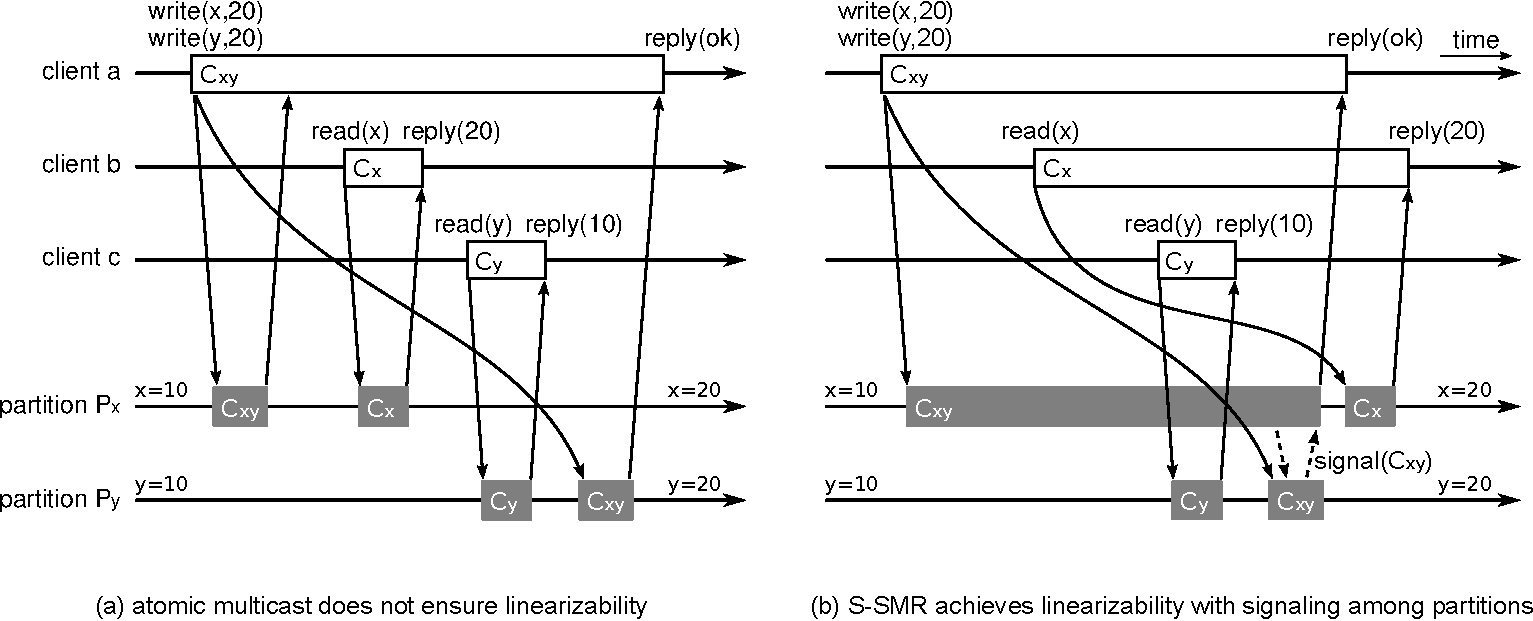
\includegraphics[width=1\linewidth]{figures/ssmr}
  \end{minipage}
  \caption{Atomic multicast and S-SMR. (To simplify the figure, we show a single replica per partition.)}
  \label{fig:ssmr}
\end{figure*}

To execute a command, the client multicasts the command to the appropriate
partitions, as determined by the oracle. Commands that access a single partition
are executed as in classical SMR: replicas of the concerned partition agree on
the execution order and each replica executes the command independently. In the
case of a multi-partition command, replicas of the involved partitions deliver
the command and then may need to exchange state in order to execute the command
since some partitions may not have all the values read in the command. This
mechanism allows commands to execute seamlessly despite the partitioned state.

S-SMR improves on classical SMR by allowing replicated systems to scale, while
ensuring linearizability. Under workloads with multi-partition commands,
however, it has limited performance, in terms of latency and throughput
scalability. Such decreased performance when executing multi-partition commands
is due to partitions (i) exchanging state variables and (ii) synchronizing by
exchanging signals. Thus, the performance of \ssmr\ is particularly
sensitive to the way the service state is partitioned.

One way to reduce the number of multi-partition commands is by dynamically
changing the partitioning, putting variables that are usually accessed together
in the same partition. However, the partitioning oracle of \ssmr\ relies on a
static mapping of variables to partitions. One advantage of this implementation
is that all clients and servers can have their own local oracle, which always
returns a correct set of partitions for every query. Such a static mapping has
the major limitation of not allowing the service to dynamically adapt to
different access patterns.

\subsection{Two phases locking and two phases commit with Google Spanner}

Google Spanner~\cite{corbett2013spanner} was designed to be a highly-scalable
distributed relational database. Spanner consists of multiple \emph{zones}, each
of which is a deployment of Bigtable servers. A zone uses one \emph{zonemaster}
to assign data to one hundred to several thousand sets of Paxos-based state
machines (so called \emph{spanservers}). Clients in Spanner use \emph{location
proxy} of each zone to locate the spanservers assigned to serve their data.
Although not detailed in the paper, Spanner allows data to be re-sharded across
\emph{spanservers} or \emph{zones} data centers to balance loads and in response
to failures by \emph{placement driver}. Periodically, \emph{placement driver}
communicates with spanservers tor re-arrange data. During these transfers,
clients can still execute transactions (including updates) on the database.
Figure~\ref{fig:spanner} shows an execution of a single transactions that
requires multiple round of coordination in Spanner.

\begin{figure*}
  \begin{minipage}[b]{1.0\linewidth}
  \centering
        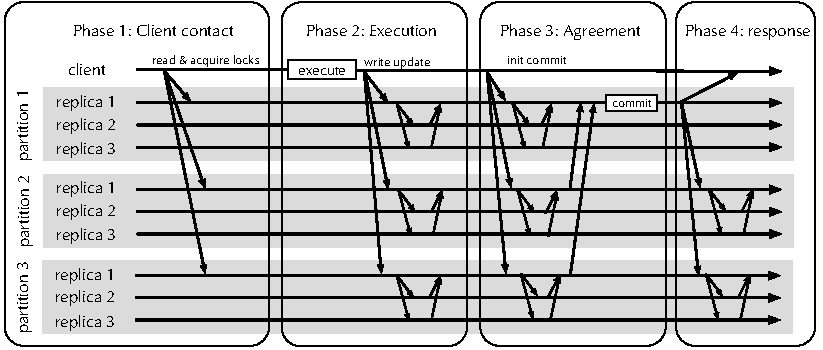
\includegraphics[width=0.6\linewidth]{figures/spanner}
  \end{minipage}
  \caption{Coordination required in multi-partition transaction in Spanner}
  \label{fig:spanner}
\end{figure*}

\section{Workload graph partitioning}

%\ssmr\ performs better as the number of multi-partition commands decreases.




% Static techniques choose an immutable assignment of application state variables
% to partitions prior to executing commands. Dynamic techniques address the
% limitations of static techniques by adapting the partitioning scheme as
% workloads change. For example, a dynamic technique can move data ``on demand''
% to maximize the number of single partition user commands, while avoiding
% imbalances in the load of the partitions.
% %Typically, this is implemented by moving data ``on demand'' to a single
% %partition which executes a user command.
% The major challenge in designing a dynamic scheme is determining how the system
% selects the partition to which to move data.


% Figure~\ref{fig:motivation} shows the result of a motivating experiment that
% compares two representative systems, one of each class. In the experiment, we
% measured the throughput and number of state moves over time with two different
% workloads: one with strong locality and one with weak locality. The workloads
% are inspired by the social network Twitter, in which the network is modeled as a
% graph, and users can ``post'' messages. The social graph was generated using a
% Zipfian distribution, where the Zipf parameter was adjusted to alter the
% locality.  For brevity, we postpone the details of the experimental setup until
% Section~\ref{sec:experiments}.


% Static techniques choose an immutable assignment of application state variables
% to partitions prior to executing commands. As an example of a static approach
% for use in the experiment, we modified the S-SMR system~\cite{bezerra2014ssmr}
% to use the static METIS~\cite{Abou-Rjeili:2006} partitioning algorithm.  The
% METIS algorithm is optimized to minimize edge-cuts when partitioning a static
% social graph. In the workload with strong locality, METIS partitions the social
% graph such that all posts are single partition; in the workload with weak
% locality, although most commands are single partition, a small fraction of posts
% involves multiple partitions. The throughput is less for the weak locality
% workload due to the more expensive execution of multi-partition posts.
% %since the static scheme incurs overhead when accessing multiple partitions to
% %execute commands.
% For workloads that do not change the graph structure and exhibit strong
% locality, the results for optimized S-SMR in Figure~\ref{fig:motivation} show a
% theoretical maximum throughput.  Of course, these results are not achievable in
% practice, since for real workloads, the graph would change over time (e.g., in
% social networks users join and leave the system, connections are created and
% removed).


% Dynamic techniques address the limitations of static techniques by adapting the
% partitioning scheme as workloads change. For example, a dynamic technique can
% move data ``on demand'' to maximize the number of single partition user
% commands, while avoiding imbalances in the load of the partitions.
% %Typically, this is implemented by moving data ``on demand'' to a single
% %partition which executes a user command.
% The major challenge in designing a dynamic scheme is determining how the system
% selects the partition to which to move data.
% %
% The second system in Figure~\ref{fig:motivation} evaluates DS-SMR, a dynamic
% partitioning strategy implemented by  Le et al.~\cite{hoang2016}. This system
% selects partitions randomly, which allows for a completely decentralized
% implementation, in which partitions make only local choices about data movement.
% We refer to this approach as \emph{decentralized dynamic}.  As
% Figure~\ref{fig:motivation} shows, the decentralized dynamic approach works well
% for data with strong locality, but is unstable for workloads with weak locality,
% since data is constantly moved from one partition to another.



% \subsection{Scalable state-machine replication}


\chapter[Dynamic partitioning for SMR]{Dynamic partitioning for SMR}
\label{sec:dssmr}
% \section{Limitation of static partitioned SMR} \label{sec:ssmrproblem}


An inherent problem of traditional SMR is that it is not scalable: any replica
added to the system will deliver all requests, so throughput is not increased.
Scalable SMR addresses this issue in two ways: (i) by partitioning the
application state, while allowing every command to access (read/write) any
combination of partitions and (ii) using caching to reduce the communication
across partitions, while keeping the execution linearizable.

On the downside of this approach, as the number of multi-partition commands
increases, performance of \ssmr\ decreases, as partitions must communicate.
One way to reduce the number of multi-partition commands is by dynamically
changing the partitioning, placing variables that are usually accessed together
in the same partition. However, the partitioning oracle of \ssmr\ relies on a
static mapping of variables to partitions. One advantage of this approach
is that all clients and servers can have their own local oracle, which always
returns a correct set of partitions for every query. Such a static mapping has
the major limitation of not allowing the service to dynamically adapt to
different access patterns. Any state reorganization requires system shutdown and
manual intervention.

Given these issues, it is crucial that highly available partitioned systems be
able to dynamically adapt to the workload. In this chapter, we present
\dssmrlong\ (\dssmr), a technique that allows a partitioned SMR system to
reconfigure its data placement on-the-fly. \dssmr\ achieves dynamic data
reconfiguration without sacrificing scalability or violating the properties of
classical SMR. These requirements introduce significant challenges. Since state
variables may change location, clients must find the current location of
variables.
% The scalability requirement rules out the use of a centralized oracle that
% clients can consult to find out the partitions a command must be multicast to.
If there exists a centralized oracle that clients can consult to find out the
partitions a command must be multicast to, the system is still unlikely to
scale, as the oracle will likely become a bottleneck. Even if clients can
determine the current location of the variables needed to execute a command, by
the time the command is delivered at the involved partitions, one or more
variables may have changed their location. Although the client can retry the
command with the new locations, how to guarantee that the command will succeed
in the second attempt? In classical SMR, every command invoked by a non-faulty
client always succeeds. \dssmr\ should provide similar guarantees.

\dssmr\ was designed to exploit workload locality. Our scheme benefits from
simple manifestations of locality, such as commands that repeatedly access the
same state variables, and more complex manifestations, such as structural
locality in social network applications, where users with common interests have
a higher probability of being interconnected in the social graph. Focusing on
locality allows us to adopt a simple but effective approach to state
reconfiguration: whenever a command requires data from multiple partitions, the
variables involved are moved to a single partition and the command is executed
in this partition. To reduce the chances of skewed load among partitions,
the destination partition is chosen randomly. Although \dssmr\ could use more
sophisticated forms of partitioning, formulated as an optimization problem
(e.g., \cite{curino2010sch,taft2014est}), our technique has the advantage that
it does not need any prior information about the workload and is not
computationally expensive.

To track object locations without compromising scalability, in addition to a
centralized oracle that contains accurate information about the location of
state variables, each client caches previous consults to the oracle. As a
result, the oracle is only contacted the first time a client accesses a variable
or after a variable changes its partition. Under the assumption of locality, we
expect that most queries to the oracle will be accurately resolved by the
client's cache. To ensure that commands always succeed, despite concurrent
relocations, after attempting to execute a command a few times unsuccessfully,
\dssmr\ retries the command using \ssmr{}'s execution atomicity and involving
all partitions. Doing so increases the cost to execute the command but
guarantees that relocations will not interfere with the execution of the
command.

We have fully implemented \dssmr\ as the \dssmrlibname{} Java library, and we
performed a number of experiments using \dssmrappname{}, a social network
application built with \dssmrlibname{}. We compared the performance of \dssmr\
to \ssmr\ using different workloads. With a mixed workload that combines various
operations issued in a social network application, \dssmr\ reached 74~kcps
(thousands of commands per second), against less than 33~kcps achieved by
\ssmr{}, improving by a factor of over 2.2. Moreover, \dssmr's performance
scales with the number of partitions under all workloads.

The following contributions are presented in this chapter:
(1) It introduces \dssmr\ and discusses some performance optimizations, including
the caching technique.
(2) It details \dssmrlibname{}, a Java library to simplify the design of services based
on \dssmr{}.
(3) It describes \dssmrappname{} to demonstrate how \dssmrlibname{} can be used to implement
a scalable social network service.
(4) It presents a detailed experimental evaluation of \dssmrappname{}, deploying it with
\ssmr\ and \dssmr{} in order to compare the performance of the two replication
techniques.

The remainder of this chapter is organized as follows.
Section \ref{sec:dssmr-idea} gives an overview of DS-SMR.
Section \ref{sec:dssmr-detail} explains the algorithm in detail.
Section \ref{sec:dssmr-optm} proposes some performance optimizations.
Section \ref{sec:dssmr-correctness} argues about the correctness of the algorithm.
Section \ref{sec:dssmr-implementation} details the implementation of Eyrie.
Section \ref{sec:dssmr-experiments} reports on the performance of \dssmrlibname and Chirper.
Section \ref{sec:dssmr-conclusion} concludes the chapter.

\section{General idea}
\label{sec:dssmr-idea}

Dynamic \ssmr\ (\dssmr) defines a dynamic mapping of variables to partitions.
Each variable $v$ is mapped to partition $\ppm$, meaning that $v \in \ppm$. Such
a mapping is managed by a partitioning oracle, which is implemented as a
replicated service run by a group of server processes $\ssm_0$. The oracle
service allows the mapping of variables to partitions to be retrieved or changed
during execution. In more detail, \dssmr\ distinguishes five types of commands:
$access(\omega)$ is an application command that accesses (reads or writes)
variables in set $\omega \subseteq \vvm$ (as described in
Section~\ref{sec:sysmodel}), $create(v)$ creates a new variable $v$ and
initially maps it to a partition defined by the oracle, $delete(v)$ removes $v$
from the service state,
$move(v,\ppm_s,\ppm_d)$ moves variable $v$ from partition $\ppm_s$ to partition
$\ppm_d$, and $consult(C)$ asks the oracle which variables are accessed by
command $C$, and which partition contains each of them. The reply from the
oracle to a $consult$ command is called a $prophecy$. A prophecy usually
consists of a set of tuples $\langle v, \ppm \rangle$, meaning that variable $v$
is mapped to partition $\ppm$. The other possible values for a prophecy are $ok$
and $nok$, which mean that a command can and cannot be executed, respectively.

Clients can consult the oracle to know which partitions each command should be
multicast to, based on which variables are accessed by the command. If the reply
received from the oracle tells the client that the command accesses a single
partition, the client multicasts the command to that partition. If the command
accesses variables from multiple partitions, the client first multicasts one or
more $move$ commands to the oracle and to the involved partitions, with the
intent of having all variables in the same partition. Then, the command itself
is multicast to the one partition that now holds all variables accessed by the
command. If a subsequent command accesses the same variables, it will also
access a single partition. With this scheme, the access patterns of commands
will shape the mapping of variables to partitions, reducing the number of
multi-partition commands.

\begin{figure*}
\begin{minipage}[b]{1.0\linewidth}
\centering
      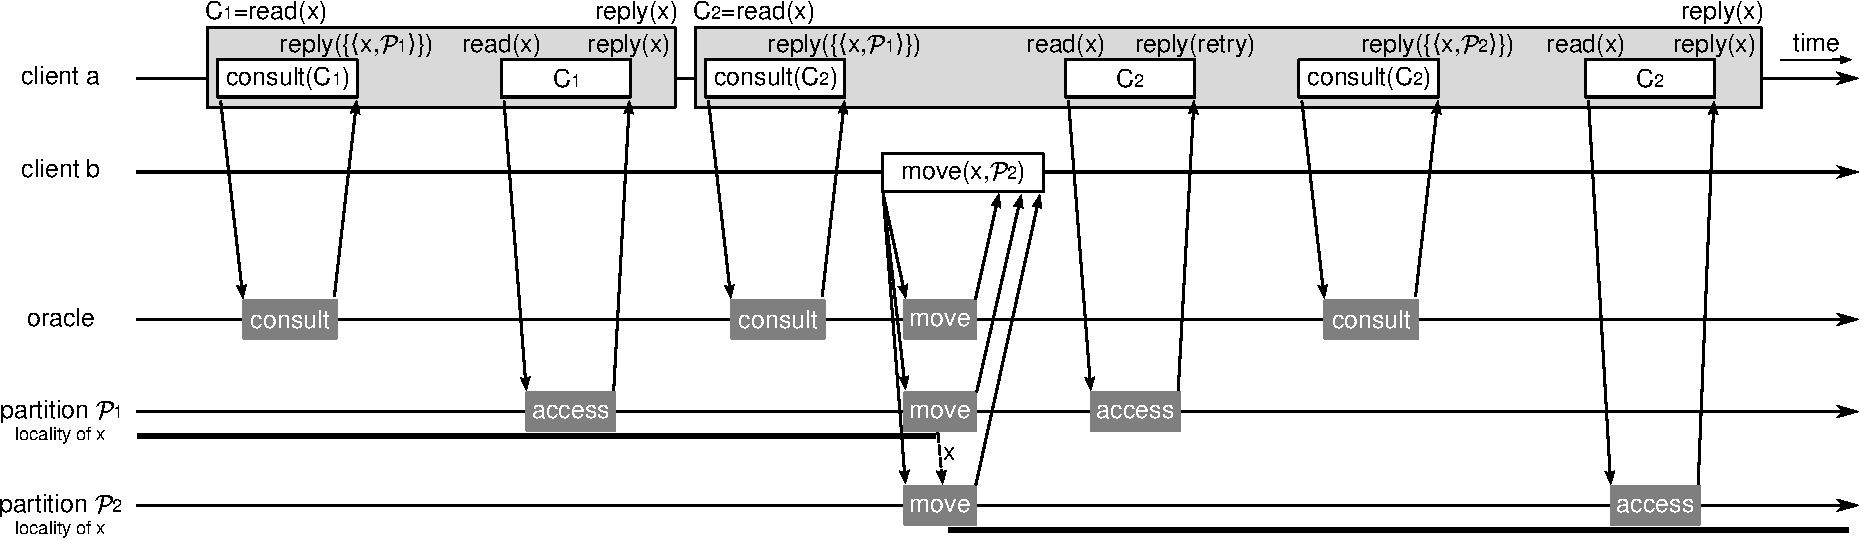
\includegraphics[width=1\linewidth]{figures/dssmr-detail}
\end{minipage}
\caption{Consulting the oracle and issuing a command are done in multiple calls to atomic multicast.}
\label{fig:dssmr-detail}
\end{figure*}

Consulting the oracle and issuing the application command are done with separate
calls to atomic multicast in \dssmr{}. It may happen that, between those
operations, the partitioning changes. We illustrate this in
Figure~\ref{fig:dssmr-detail}. Commands $C_1$ and $C_2$ read variable $x$. Since
partitioning is dynamic, the client issuing the commands first consults the
oracle before multicasting each command. $C_1$ executes without the interference
of other commands, so consulting the oracle and multicasting the command only
once is enough for $C_1$ to be executed. However, before $C_2$ is multicast to
$\ppm_1$, another client issues a $move$ command that relocates $x$ to $\ppm_2$.
When $C_2$ is delivered at the servers of $\ppm_1$, the command is not executed,
since $x$ is not available at $\ppm_1$ anymore. A similar situation may arise
when a command accesses variables from multiple partitions, as it consists of
multicasting at least three commands separately: $consult$, $move$ and $access$.
The partitioning can change between the execution of any two of those commands.

To solve this problem, the client multicasts the set of variables accessed along
with each access command. Upon delivery, each server checks the set of variables
sent by the client. If all variables in the set belong to the local partition,
the command is executed; otherwise, a $retry$ message is sent back to the
client. When the client receives a $retry$ message, it consults the oracle
again, possibly moving variables across partitions, and then reissues the access
command. To guarantee termination, if the command fails a certain number of
times, the client multicasts the command to all partitions and the servers
execute it as in the original \ssmr{}.

The \dssmr\ client consists of the application logic and a client proxy.
The application does not see the state variables divided into partitions. When
the application issues a command, it sends the command to the proxy and
eventually receives a reply. All commands that deal with partitioning (i.e.,
consulting the oracle, moving objects across partitions and retrying commands as
described in the previous paragraph) are executed by the client proxy,
transparently to the application. When the client proxy multicasts a
partitioning-related command to multiple partitions and the oracle, partitions
and oracle exchange signals to ensure linearizability, as mentioned in
Section~\ref{sec:ssmr}. Every server and oracle process has their own \dssmr\
proxy as well. At each server, the proxy checks whether commands can be executed
and manages the exchange of data and signals between processes. At the oracle,
the service designer defines the application-dependent rules that must be
followed (e.g., where each variable is created at first) and a proxy is
responsible for managing the communication of the oracle with both clients and
servers when executing commands. \dssmr\ relies on a fault-tolerant multicast
layer for disseminating commands across replicas and implementing reliable
communication between partitions. Replies to commands are sent directly through
the network. Figure~\ref{fig:dssmr-arch} illustrates the architecture of \dssmr{}.

\begin{figure*}
\begin{minipage}[b]{1.0\linewidth}
\centering
      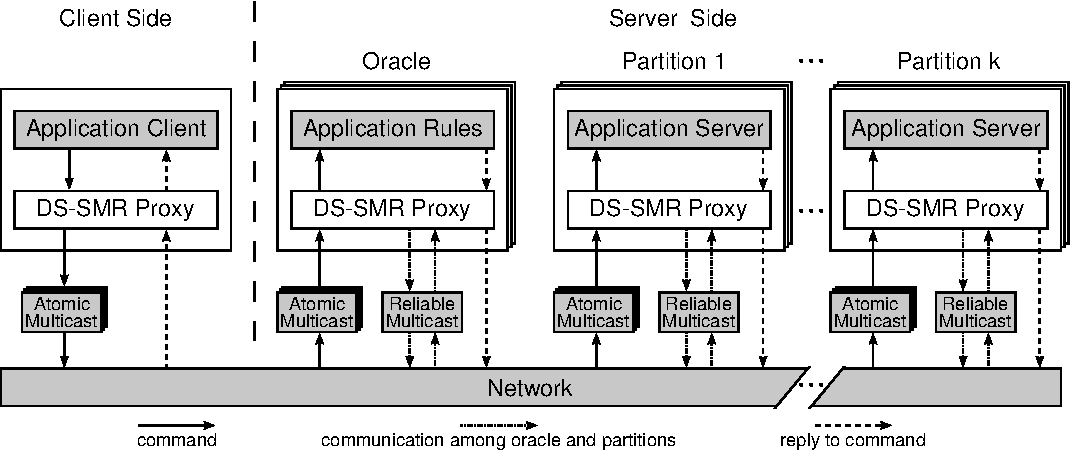
\includegraphics[width=0.8\linewidth]{figures/dssmr-arch}
\end{minipage}
\caption{The architecture of \dssmrlong{}.}
\label{fig:dssmr-arch}
\end{figure*}


\section{Detailed algorithm}
\label{sec:dssmr-detail}


When issuing a command, the application simply forwards the command to the
client proxy and waits for the reply. Consulting the oracle and multicasting the
command to different partitions is done internally by the proxy at the client.
Algorithms~\ref{alg:client_proxy}, \ref{alg:server_proxy}, and
\ref{alg:oracle_proxy} describe in detail how the \dssmr\ proxy works
respectively at client, server and oracle processes. Every server proxy at a
server in $\ssm_i$ has only partial knowledge of the partitioning: it knows only
which variables belong to $\ppm_i$. The oracle proxy has knowledge of every
$\ppm \in \Psi$. To maintain such a global knowledge, the oracle must \amdel{}
every command that creates, moves, or deletes variables. (In
Section~\ref{sec:dssmr-optm}, we introduce a caching mechanism to prevent the oracle
from becoming a performance bottleneck.)

\begin{algorithm}[t!]
\small

\begin{distribalgo}[1]

\vspace{1.0mm}

\INDENT{To issue a command $C$, the client proxy does:}

\vspace{1.0mm}

    \INDENT{\textbf{do}}
        \STATE \amcast$($oracle, $consult(C))$
        \STATE wait for $prophecy$
        \IF{$prophecy \in \{ok, nok\}$}
            \STATE $reply \leftarrow prophecy$
        \ELSE
            \STATE $C.dests \leftarrow \{\ppm : \exists \langle v, \ppm \rangle \in prophecy \}$
            \IF{$C$ is an $access(\omega)$ command and $|C.dests| > 1$}
                \STATE let $\ppm_d$ be one of the partitions in $C.dests$
                \label{algline:client:partition}
                \FOR{each $v \in \omega$}
                    \STATE // \textit{move $v$ to partition $\ppm_d$}
                    \STATE let $\ppm_s$ be $\ppm : \langle v, \ppm \rangle \in prophecy$
                    \IF{$\ppm_s \neq \ppm_d$}
                        \STATE $C_{move} \leftarrow move(v,\ppm_s,\ppm_d)$
                        \STATE $C_{move}.dests \leftarrow \{$oracle$,\ppm_s,\ppm_d\}$    
                        \STATE \amcast$(C_{move}.dests$, $C_{move})$
                    \ENDIF
                \ENDFOR
                \STATE $C.dests \leftarrow \{ \ppm_d \}$
            \ENDIF
            \IF{$C$ is $create$ or $delete$}
                \STATE $C.dests \leftarrow dests \cup \{oracle\}$
            \ENDIF
            \STATE \amcast$(C.dests$, $C)$
            \STATE wait for $reply$
        \ENDIF
    \ENDINDENT
    \STATE{\textbf{while} $reply = retry$ // \textit{after many retries, fall back to \ssmr}}
    \STATE return $reply$ to the application client
\ENDINDENT

\caption{\dssmr\ Client Proxy}
\label{alg:client_proxy}
\end{distribalgo}
\end{algorithm}
\fxnote{Clarifying algorithm}
\textbf{The client proxy.} To execute a command $C$, the proxy first consults
the oracle. The oracle knows all state variables and which partition contains
each of them. Because of this, the oracle may already tell the client whether
the command can be executed or not. Such is the case of the $access(\omega)$
command: if there is a variable $v \in \omega$ that the command tries to read or
write and $v$ does not exist, the oracle already tells the client that the
command cannot be executed, by sending $nok$ as the prophecy. A $nok$ prophecy
is also returned for a $create(v)$ command when $v$ already exists. For a
$delete(v)$ command when $v$ already does not exist, an $ok$ prophecy is
returned. If the command can be executed, the client proxy receives a prophecy
containing a pair $\langle v, \ppm \rangle$, for every variable $v$ created,
accessed or deleted by the command. \lle{If the prophecy regarding an
$access(\omega)$ command contains multiple partitions, the client proxy randomly chooses
one of them,} $\ppm_d$, and tries to move all variables in $\omega$ to $\ppm_d$.
Then, the command $C$ itself is multicast to $\ppm_d$. As discussed in
Section~\ref{sec:dssmr-idea}, there is no guarantee that an interleave of
commands will not happen, even if the client waits for the replies to the move
commands. For this reason, and to save time, the client proxy multicasts all
move commands at once. Commands that change the partitioning (i.e., create and
delete) are also multicast to the oracle. If the reply received to the command
is $retry$, the procedure restarts: the proxy consults the oracle again,
possibly moves variables across partitions, and multicasts $C$ to the
appropriate partitions once more. After reaching a given threshold of retries
for $C$, the proxy falls back to \ssmr{}, multicasting $C$ to all partitions
(and the oracle, in case $C$ is a create or delete command), which ensures the
command's termination.

\begin{algorithm}[t!]
\small

\begin{distribalgo}[1]

\vspace{1.0mm}

\INDENT{To execute a command $C$, the server proxy in partition $\ppm$ does:}

    \vspace{1.0mm}
    
    \INDENT{\textbf{when} \rmdel$( \langle val, C \rangle )$}
        \STATE $rcvd\_msgs \leftarrow rcvd\_msgs \cup \{\langle val, C \rangle\}$
    \ENDINDENT

    \vspace{1.0mm}

    \INDENT{\textbf{when} \amdel$(C)$}

    \vspace{1.0mm}

        \IF{\underline{$C$ is an $access(\omega)$ command}}
            \IF{$\exists v \in \omega : v \not\in \ppm$}
                \STATE reply with $retry$
            \ELSE
                \STATE have the command executed by the application server
                \STATE send the reply to the client
            \ENDIF
        

        \vspace{1.0mm}
    
        \ELSIF{\underline{$C$ is a $move(v,\ppm_s,\ppm_d)$ command}}
            \IF{$\ppm = \ppm_s$}
                \IF{$v \in \ppm$}
                    \STATE \rmcast$(\ppm_d$,$\langle v, C \rangle)$
                    \STATE $\ppm \leftarrow \ppm \setminus \{v\}$
                \ELSE
                    \STATE \rmcast$(\ppm_d$,$\langle null, C \rangle)$
                \ENDIF
            \ELSE
                \STATE wait until $\exists val : \langle val, C \rangle \in rcvd\_msgs$
                \IF{$val \neq null$}
                    \STATE $v \leftarrow val$
                    \STATE $\ppm \leftarrow \ppm \cup \{v\}$
                \ENDIF
            \ENDIF
        
        \vspace{1.0mm}
    
        \ELSIF{\underline{$C$ is a $create(v)$ command}}
            \STATE wait until $\langle val, C \rangle \in rcvd\_msgs$
            \IF{$val = ok$}
                \STATE $\ppm \leftarrow \ppm \cup \{v\}$
%                \STATE reply with $success$
%            \ELSE
%                \STATE reply with $retry$
            \ENDIF
        
        \vspace{1.0mm}
        
        \ELSIF{\underline{$C$ is a $delete(v)$ command}}
            \IF{$v \in \ppm$}
                \STATE $\ppm \leftarrow \ppm \setminus \{v\}$
%                \STATE reply with $success$
%            \ELSE
%                \STATE reply with $retry$
            \ENDIF
        \ENDIF
    \ENDINDENT
\ENDINDENT

\caption{\dssmr\ Server Proxy}
\label{alg:server_proxy}
\end{distribalgo}
\end{algorithm}

\textbf{The server proxy.} Upon delivery, access commands are intercepted by the
\dssmr\ proxy before they are executed by the application server. In \dssmr{},
every access command is executed in a single partition. If a server proxy in
partition $\ppm$ intercepts an $access(\omega)$ command that accesses a variable
$v \in \omega$ that does not belong to $\ppm$, it means that the variable is in
some other partition, or it does not exist. Either way, the client should retry
with a different set of partitions, if the variable does exist. To execute a
$delete(v)$ command, the server proxy at partition $\ppm$ simply removes $v$
from partition $\ppm$, in case $v \in \ppm$. In case $v \not\in \ppm$, it might
be that the variable exists but belongs to some other partition $\ppm'$. Since
only the oracle and the servers at $\ppm'$ have this knowledge, it is the oracle
who replies to delete commands.

The \dssmr\ server and oracle proxies coordinate to execute commands that create or
move variables. Such coordination is done by means of \rmcast{}. When a
$create(v)$ command is delivered at $\ppm$, the server proxy waits for a message
from the oracle, telling whether the variable can be created or not, to be
\rmdel{}ed. Such a message from the oracle is necessary because $v$ might not
belong to $\ppm$, but it might belong to some other partition $\ppm'$ that
servers of $\ppm$ have no knowledge of. If the create command can be executed,
the oracle can already reply to the client with a positive acknowledgement,
saving time. This can be done because atomic multicast guarantees that all
non-faulty servers at $\ppm$ will eventually deliver and execute the command. As
for move commands, each $move(v,\ppm_s,\ppm_d)$ command consists of moving
variable $v$ from a source partition $\ppm_s$ to a destination partition
$\ppm_d$. If the server's partition $\ppm$ is the source partition (i.e., $\ppm$
= $\ppm_s$), the server proxy checks whether $v$ belongs to $\ppm$. If $v \in
\ppm$, the proxy \rmcast{}s $\langle v, C \rangle$ to $\ppm_d$, so that servers
at the destination partition know the most recent value of $v$; $C$ is sent
along with $v$ to inform which move command that message is related to. If $v
\not\in \ppm$, a $\langle null, C \rangle$ message is \rmcast\ to $\ppm_d$,
informing $\ppm_d$ that the move command cannot be executed.

\begin{algorithm}[t!]
\small

\begin{distribalgo}[1]

\vspace{1.5mm}

\INDENT{To execute a command $C$, the oracle proxy does:}

    \vspace{1.5mm}

    \INDENT{\textbf{when} \amdel$(C)$}

    \vspace{1.5mm}

        \IF{\underline{$C$ is a $consult(C_c)$ command}}
            \STATE $prophecy \leftarrow \emptyset$

            \IF{$C_c$ is an $access(\omega)$ command}
                \IF{$\exists v \in \omega : (\nexists \ppm \in \Psi : v \in \ppm)$}
                    \STATE $prophecy \leftarrow nok$
                \ELSE
                    \FOR{each $v \in \omega$}
                        \STATE $prophecy \leftarrow prophecy \cup \{\langle v, \ppm \rangle \}:v \in \ppm$
                    \ENDFOR
                \ENDIF

            \ELSIF{$C_c$ is a $create(v)$ command}
                \IF{$\exists \ppm \in \Psi : v \in \ppm$}
                    \STATE $prophecy \leftarrow nok$
                \ELSE
                    \STATE $\ppm \leftarrow$ initial partition, defined by application rules
                    \STATE $prophecy \leftarrow \{\langle v, \ppm \rangle \}$
                \ENDIF

            \ELSIF{$C_c$ is a $delete(v)$ command}
                \IF{$\nexists \ppm \in \Psi : v \in \ppm$}
                    \STATE $prophecy \leftarrow ok$
                \ELSE
                    \STATE $prophecy \leftarrow \{\langle v, \ppm \rangle \} : v \in \ppm$
                \ENDIF
                
            \ENDIF
            
            \STATE send $prophecy$ to the client

        \vspace{1.5mm}

        \ELSIF{\underline{$C$ is a $move(v,\ppm_s,\ppm_d)$ command}}
            \IF{$v \in \ppm_s$}
                \STATE $\ppm_s \leftarrow \ppm_s \setminus \{v\}$
                \STATE $\ppm_d \leftarrow \ppm_d \cup      \{v\}$
            \ENDIF

        \vspace{1.0mm}
    
        \ELSIF{\underline{$C$ is a $create(v)$ command}}
            \STATE let $\ppm_c$ be $\ppm : \{\ppm\} = C.dests \setminus \{$oracle$\}$
            \IF{$\nexists \ppm \in \Psi : v \in \ppm$}
                \STATE $outcome \leftarrow ok$
            \ELSE
                \STATE $outcome \leftarrow nok$
            \ENDIF
            \STATE \rmcast$(\ppm_c, \langle outcome, C \rangle )$
            \STATE send $outcome$ to the client
        
        \vspace{1.0mm}
        
        \ELSIF{\underline{$C$ is a $delete(v)$ command}}
            \STATE let $\ppm_d$ be $\ppm : \{\ppm\} = C.dests \setminus \{$oracle$\}$
            \IF{$\nexists \ppm \in \Psi: v \in \ppm$ or $v \in \ppm_d$}
                \STATE send $ok$    to the client
            \ELSE
                \STATE send $retry$ to the client
            \ENDIF
            
            
        \ENDIF
    \ENDINDENT
\ENDINDENT

\caption{\dssmr\ Oracle Proxy}
\label{alg:oracle_proxy}
\end{distribalgo}
\end{algorithm}

\textbf{The oracle proxy.} One of the purposes of the oracle proxy is to make
prophecies regarding the location of state variables. Such prophecies are used
by client proxies to multicast commands to the right partitions. A prophecy
regarding an $access(\omega)$ command contains, for each $v \in \omega$, a pair
$\langle v, \ppm \rangle$, meaning that $v \in \ppm$. If any of the variables in
$\omega$ does not exist, the prophecy already tells the client that the command
cannot be executed (with a $nok$ value). For a $create(v)$ command, the prophecy
tells where $v$ should be created, based on rules defined by the application, if
$v$ does not exist. If $v$ already exists, the prophecy will contain $nok$, so
that the client knows that the create command cannot be executed. The prophecy
regarding a $delete(v)$ command has the partition that contains $v$, or
$ok$, in case $v$ was already deleted or never~existed.

Besides dispensing prophecies, the oracle is responsible for executing create,
move, and delete commands, coordinating with server proxies when necessary, and
replying directly to clients in some cases. For each $move(v,\ppm_s,\ppm_d)$
command, the oracle checks whether $v$ in fact belongs to the source partition
$\ppm_s$. If that is the case, the command is executed, moving $v$ to $\ppm_d$.
Each $create(v)$ command is multicast to the oracle and to a partition $\ppm$.
If $v$ already exists, the oracle tells $\ppm$ that the command cannot be
executed, by \rmcast{}ing $nok$ to $\ppm$. The oracle also sends $nok$ to the
client as reply, meaning that $v$ already exists. If $v$ does not exist, the
oracle tells $\ppm$ that the command can be executed, by \rmcast{}ing $ok$ to
$\ppm$. It also tells the client that the command succeeded with an $ok$ reply.
Finally, each $delete(v)$ command is multicast to the oracle and to a partition
$\ppm$, where the client proxy assumed $v$ to be located. If $v$ belongs to
$\ppm$, or $v$ does not exist, the oracle tells the client that the delete
command succeeded. Otherwise, that is, if $v$ exists, but $delete(v)$ was
multicast to the wrong partition, the oracle tells the client to retry.



\section{Performance optimizations}
\label{sec:dssmr-optm}

In this section, we introduce two optimizations for \dssmr{}: caching and load
balancing.

\textbf{Caching.} In Algorithm~\ref{alg:client_proxy}, for every command issued
by the client, the proxy consults the oracle. If every command passes by the
oracle, the system is unlikely to scale, as the oracle is prone to becoming a
bottleneck. To provide a scalable solution, each client proxy has a local cache
of the partitioning information. Before multicasting an application command $C$
to be executed, the client proxy checks whether the cache has information about
every variable concerned by $C$. If the cache does have such a knowledge, the
oracle is not consulted and the information contained in the cache is used
instead. If the reply to $C$ is $retry$, the oracle is consulted and the
returned prophecy is used to update the client proxy's cache.
Algorithm~\ref{alg:client_proxy} is followed from the second attempt to execute
$C$ on. The cache is a local service that follows an algorithm similar to that
of the oracle, except it responds only to $consult(C)$ commands and, in
situations where the oracle would return $ok$ or $nok$, the cache tells the
client proxy to consult the actual oracle.


Naturally, the cached partitioning information held by the client proxy may be
outdated. On the one hand, this may lead a command to be multicast to the
wrong set of partitions, which will incur in the client proxy having to
retry executing the command. For instance, in Figure~\ref{fig:dssmr-retry} the
client has an outdated cache, incurring in a new consultation to the oracle
when executing $C_3$. On the other hand, the client proxy may already have to
retry commands, even if the oracle is always consulted first, as shown in
Figure~\ref{fig:dssmr-detail}. If most commands are executed without consulting
the oracle, as in the case of $C_4$ in Figure~\ref{fig:dssmr-retry}, we avoid
turning the oracle into a bottleneck. Moreover, such a cache can be updated
ahead of time, not having to wait for an actual application command to be issued
to only then consult the oracle. This way, the client proxy can keep a cache of
partitioning information of variables that the proxy deems likely to be accessed
in the future.

\textbf{Load balancing}. When moving variables, the client proxies may try to
distribute them in a way that balances the workload among partitions. This way,
the system is more likely to scale throughput with the number of server groups.
One way of balancing load is by having roughly the same number of state
variables in every partition. This can be implemented by having client proxies
choosing randomly the partition that will receive all variables concerned by
each command (at line~\ref                {algline:client:partition} of
Algorithm~\ref{alg:client_proxy}). Besides improving performance, balancing the
load among partitions prevents the system from degenerating into a
single-partition system, with all variables being moved to the same place as
commands are executed.


\begin{figure*}
\begin{minipage}[b]{1\linewidth} % A minipage that covers the whole width of the
page
\centering
      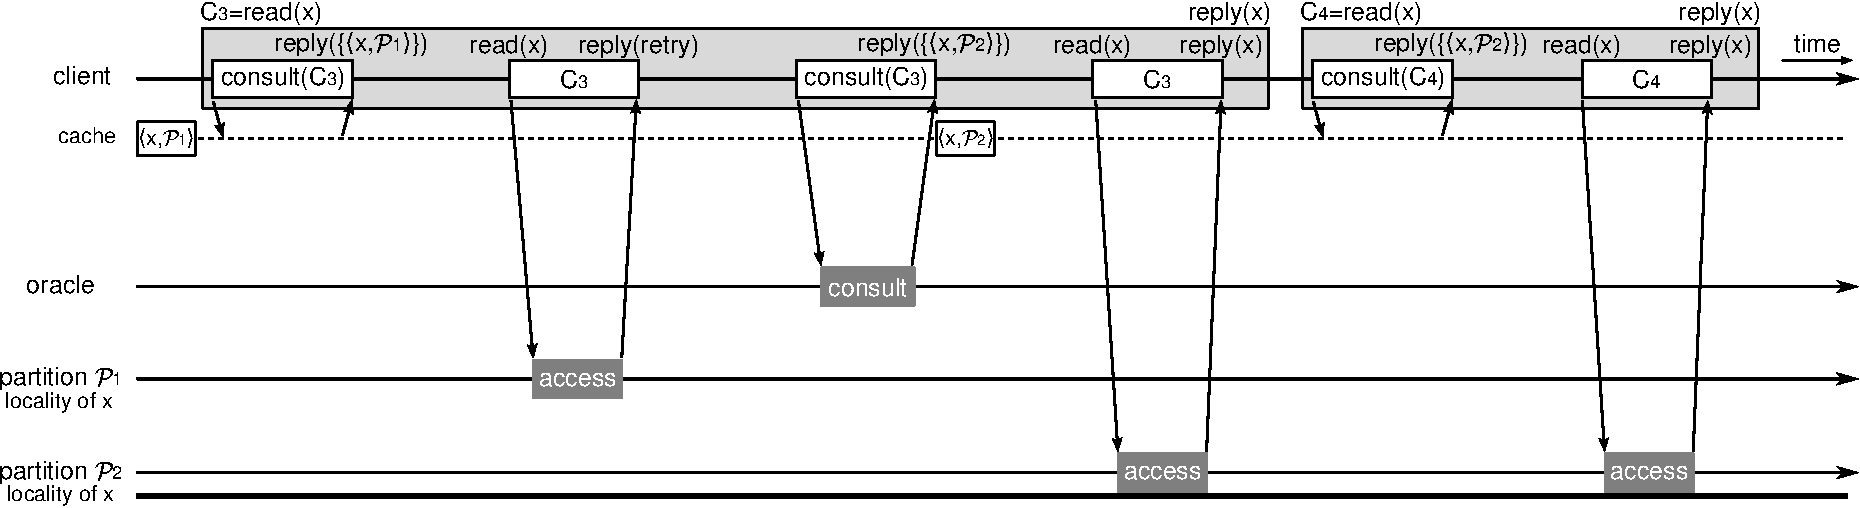
\includegraphics[width=1.0\linewidth]{figures/dssmr-retry}
\end{minipage}
\caption{Each client proxy in \dssmr\ maintains a cache in order to avoid  consulting the oracle. White boxes represent actions of the client proxy.}
\label{fig:dssmr-retry}
\end{figure*}


\section{Correctness}
\label{sec:dssmr-correctness}

In this section, we argue that \dssmr\ ensures termination and linearizability.
By ensuring termination, we mean that for every command $C$ issued by a correct
client, a reply to $C$ different than $retry$ is eventually received by the
client. This assumes that at least one oracle process is correct and that every
partition has at least one correct server. Given these constraints, the only
thing that could prevent a command from terminating would be an execution that
forced the client proxy to keep retrying a command. This problem is trivially
solved by falling back to \ssmr\ after a predefined number of retries: at a
certain point, the client proxy multicasts the command to all server and oracle
processes, which execute the command as in \ssmr{}, i.e., with coordination
among all partitions and the oracle.

As for linearizability, we argue that, if every command in execution \ex\ of
\dssmr\ is delivered by atomic multicast and is \emph{execution atomic} (as
defined in~\cite{bezerra2014ssmr}), then \ex\ is linearizable. We denote the
order given by atomic multicast by relation $\prec$. Given any two messages
$m_1$ and $m_2$, ``$m_1 \prec m_2$'' means that there exists a process that
delivers both messages and $m_1$ is delivered before $m_2$, or there is some
message $m'$ such that $m_1 \prec m'$ and $m' \prec m_2$, which can be written
as \mbox{$m_1 \prec m' \prec m_2$}.
%\fxnote[draft]{use the phrase ``there exists a process that'' }
Also, for the purposes of this proof, we consider the oracle to be a partition,
as it also \amdel{}s and executes application commands.

Suppose, by means of contradiction, that there exist two commands $x$ and $y$,
where $x$ finishes before $y$ starts, but $y \prec x$ in the execution. There
are two possibilities to be considered: (i) $x$ and $y$ are delivered by the
same process $p$, or (ii) no process delivers both $x$ and $y$.

In case (i), at least one process $p$ delivers both $x$ and $y$. As $x$ finishes
before $y$ starts, then $p$ delivers $x$, then $y$. From the properties of
atomic multicast, and since each partition is mapped to a multicast group, no
process delivers $y$, then $x$. Therefore, we reach a contradiction in this
case.

In case (ii), if there were no other commands in \ex, then the execution of $x$
and $y$ could be done in any order, which would contradict the supposition that
$y \prec x$. Therefore, there are commands $z_1, ..., z_n$ with atomic order $y
\prec z_1 \prec \cdots \prec z_n \prec x$, where some process $p_0$ (of
partition $\ppm_0$) delivers $y$, then $z_1$; some process $p_1 \in \ppm_1$
delivers $z_1$, then $z_2$, and so on: process $p_i \in \ppm_i$ delivers
$z_{i}$, then $z_{i+1}$, where $1 \leq i < n$. Finally, process $p_n \in \ppm_n$
delivers $z_n$, then $x$.

Let $z_0 = y$ and let $atomic(i)$ be the following predicate: ``For every
process $p_i \in \ppm_i$, $p_i$ finishes executing $z_i$ only after some $p_0
\in \ppm_0$ started executing $z_0$.'' We now claim that $atomic(i)$ is true for
every $i$, where $0 \leq i \leq n$. We prove our claim by induction.

%\begin{itemize}

%\item
\emph{Basis ($i=0$)}: $atomic(0)$ is obviously true, as $p_0$ can only finish
executing $z_0$ after starting executing it.

%\item
\emph{Induction step}: If $atomic(i)$, then $atomic(i+1)$. \\
Proof: Command $z_{i+1}$ is multicast to both $\ppm_i$ and $\ppm_{i+1}$. Since
$z_{i+1}$ is execution atomic, before any $p_{i+1} \in \ppm_{i+1}$ finishes
executing $z_{i+1}$, some $p_i \in \ppm_i$ starts executing $z_{i+1}$. Since
$z_i \prec z_{i+1}$, every $p_i \in \ppm_i$ start executing $z_{i+1}$ only after
finishing the execution of $z_i$. As $atomic(i)$ is true, this will only happen
after some $p_0 \in \ppm_0$ started executing $z_0$.

%\end{itemize}

As $z_n \prec x$, for every $p_n \in \ppm_n$, $p_n$ executes command $x$ only
after the execution of $z_n$ at $p_n$ finishes. From the above claim, this
happens only after some $p_0 \in \ppm_0$ starts executing $y$. This means that
$y$ ($z_0$) was issued by a client before any client received a response for
$x$, which contradicts the assumption that $x$ precedes $y$ in real-time, i.e.,
that command $y$ was issued after the reply for command $x$ was received.


\section{Implementation}
\label{sec:dssmr-implementation}

In this section, we describe \dssmrlibname{}, a library that implements both
\ssmr\ and \dssmr{}, and \dssmrappname{}, a scalable social network application
built with \dssmrlibname{}. \dssmrlibname\ and \dssmrappname\ were both
implemented in Java. \lle{Our \dssmr{} prototype uses the Ridge atomic multicast
library \cite{bezerra2015ridge}, available as open
source.\footnote{https://bitbucket.org/kdubezerra/ridge}. Ridge is a
Paxos-based atomic multicast protocol where each message is initially forwarded
to a single f distributor, whose responsibility is to propagate the message to
all other destination. Processes in Ridge alternate in the role of distributor
to utilize all bandwidth available in the system}
\fxnote{Adding details of multicast library}

\subsection{\dssmrlibname}

To implement a replicated service with \dssmrlibname{}, the developer (i.e., service
designer) must extend three classes: PRObject, StateMachine, OracleStateMachine.

\textbf{The PRObject class.} \dssmrlibname{} supports partial replication (i.e., some
objects may be replicated in some partitions, not all). Therefore, when
executing a command, a replica might not have local access to some of the
objects involved in the execution of the command. The developer informs
\dssmrlibname{} which object classes are partially replicated by extending the
PRObject class. Each object of such a class is stored either locally or remotely,
but the application code is agnostic to that. All calls to methods of such
objects are intercepted by \dssmrlibname{}, transparently to the developer.

% are you still using the aspect? do methods actually get intercepted by
% D-Eyrie?

\textbf{The StateMachine class.} This class implements the logic of the server
proxy. The application server class must extend the StateMachine class. To
execute commands, the developer must provide an implementation for the method
executeCommand(Command). The code for such a method is agnostic to the existence
of partitions. In other words, it can be exactly the same as the code used to
execute commands with classical state machine replication (i.e., full
replication). \dssmrlibname{} is responsible for handling all communication between
partitions and oracle transparently. To start the server, method
runStateMachine() is called. Method createObject() also needs to be implemented,
where the developer defines how new state objects are loaded or created.

\textbf{The OracleStateMachine class.} This class implements the logic of the
oracle proxy. It extends StateMachine, so the oracle can be deployed similarly
to a fault-tolerant partition in the original \ssmr{}. Class OracleStateMachine
has a default implementation, but the developer is encouraged to override its
methods. Method extractObject(Command) returns the set of objects accessed by
the command. It should be overridden by the application so that the client proxy
can relocate all necessary objects to a destination partition before executing
the application command.
% didn't understand this: ``in the case there are hidden objects in the command.''
Method getTargetPartition(Set$\langle$Object$\rangle$) returns a particular
partition to which objects should be moved, when they are not in the same
partition yet, in order to execute an application command that accesses those
objects. The default implementation of the method returns a random partition.
The developer can override it in order to further improve the distribution of
objects among partitions. For instance, the destination partition could be
chosen based on an attribute of the objects passed to the method.

The client proxy is implemented in class Client, which handles all communication
of the application client with the partitioned service. The client proxy
provides methods \emph{sendCreate(Command, Callback)}, \emph{sendAccess(Command,
Callback)}, and \emph{sendDelete(Command, Callback)}. The client proxy's default
behavior is to keep retrying commands (and fallback to \ssmr\ in case of too
many retries) and only call back the application client when the command has
been successfully executed. However, the developer can change this behavior by
overriding the error() method of Callback. The error() method is called when a
$retry$ reply is received.

% i don't understand what the application can actually change with the error()
% method

\subsection{\dssmrappname}

We implemented \dssmrappname{}, a social network application similar to Twitter,
using \dssmrlibname{}. Twitter is an online social networking service in which users
can post 140-character messages and read posted messages of other users. The API
consists basically of: post (user publishes a message), follow (user starts
following another user), unfollow (user stops following someone), and
getTimeline (user requests messages of all people whom the user follows).

State partitioning in \dssmrappname\ is based on users' interest. A function $f(uid)$
returns the partition that user with id $uid$ should belong to, based on the
user's interest. Function $f$ is implemented in method getObjectPlacement(User)
of class \dssmrappname{}Oracle, which extends OracleStateMachine (class User extends
PRObject). Taking into account that a typical user probably spends more time
reading messages (i.e., issuing getTimeline) than writing them (i.e., issuing
post), we decided to optimize getTimeline to be single-partition. This means
that, when a user requests his or her timeline, all messages should be available
in the partition that stores that user's data, in the form of a materialized
timeline (similarly to a materialized view in a database). To make this
possible, whenever a post request is executed, the message is inserted into the
materialized timeline of all users that follow the one that is posting. Also,
when a user starts following another user, the messages of the followed user are
inserted into the follower's materialized timeline as part of the command
execution; likewise, they are removed when a user stops following another user.
Because of this design decision, every getTimeline request accesses only one
partition, follow and unfollow requests access objects on at most two
partitions, and post requests access up to all partitions. The \dssmrappname{} client
does not need any knowledge about partitions, since it uses method
sendAccessCommand(command) of the \dssmr{} client proxy to issue its commands.

One detail about the post request is that it needs access to all users that
follow the user issuing the post.
%Thus the list of follower need to be attached in the post command. However, the
%(Chirper) client cannot know for sure who follows the user: it keeps a cache of
%followers, but such cache can become stale if a different user starts following
%the poster.
To ensure linearizability when executing a post request, the \dssmrappname\ server
overrides the extractObject(command) method to check if all followers that will
be accessed by the command are available in the local partition (i.e., the
partition of the server executing the post command). If this is the case, the
request is executed. Otherwise, the server sends a $retry(\gamma)$ message,
where $\gamma$ is the complete set of followers of the user who was posting.
Then, the \dssmrappname\ server proceeds to the next command. Upon receiving the
$retry(\gamma)$ message, the client proxy tries to move all users in $\gamma$ to
the same partition before retrying to execute the post command.


\section{Performance evaluation}
\label{sec:dssmr-experiments}

In this section, we present the results found for \dssmrappname\ with different
loads and partitionings and compare them with the original
\ssmr{}~\cite{bezerra2014ssmr}. In these experiments, we are interested in
assessing \dssmr{}'s performance with workloads that present different levels of
locality. By locality, we mean the likelihood that certain groups of data items
are accessed together (by the same command). In
Section~\ref{sec:dssmr-evaluation:setup}, we describe the environment where we
conducted our experiments. In Section~\ref{sec:dssmr-evaluation:strongloc}, we
show the results with strong-locality workloads. In
Section~\ref{sec:dssmr-evaluation:weakloc}, we show the results for
weak-locality workloads.

\begin{figure*}[ht!]
\centering
\begin{subfigure}{1\columnwidth}
      \centering
      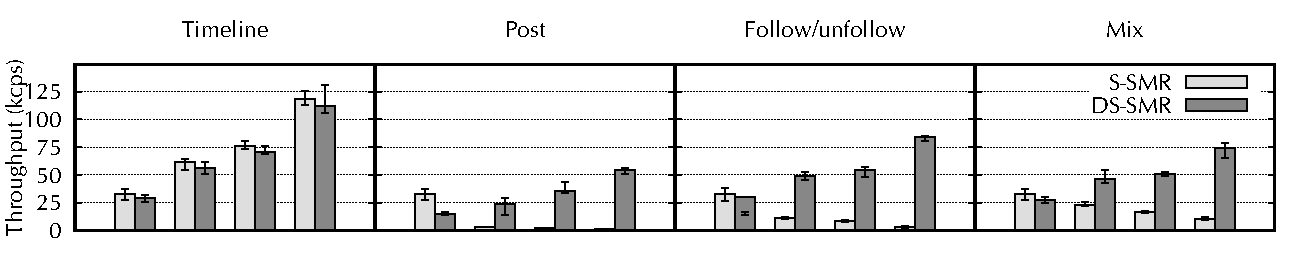
\includegraphics[width=\textwidth]{./figures/experiments/dssmr/dssmr-strong-locality-tp}
\end{subfigure}
\begin{subfigure}{1\columnwidth}
      \centering
      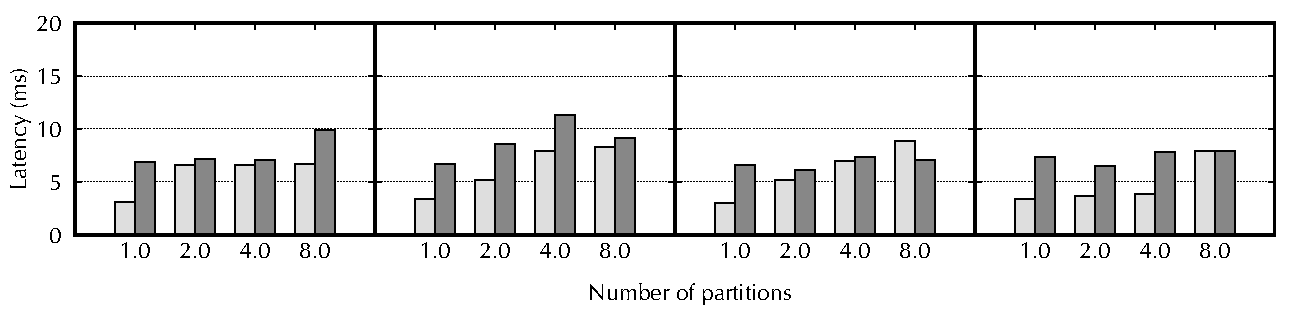
\includegraphics[width=\textwidth]{./figures/experiments/dssmr/dssmr-strong-locality-lat}
\end{subfigure}
\caption{Results of \dssmrappname\ running with \ssmr\ and \dssmr{} with strong-locality workload. Throughput is shown in thousands of commands per second (kcps).}
\label{fig:dssmr-strongloc}
\end{figure*}

% \begin{figure*}[ht!]
% \begin{minipage}[b]{1\linewidth}
% \centering
%       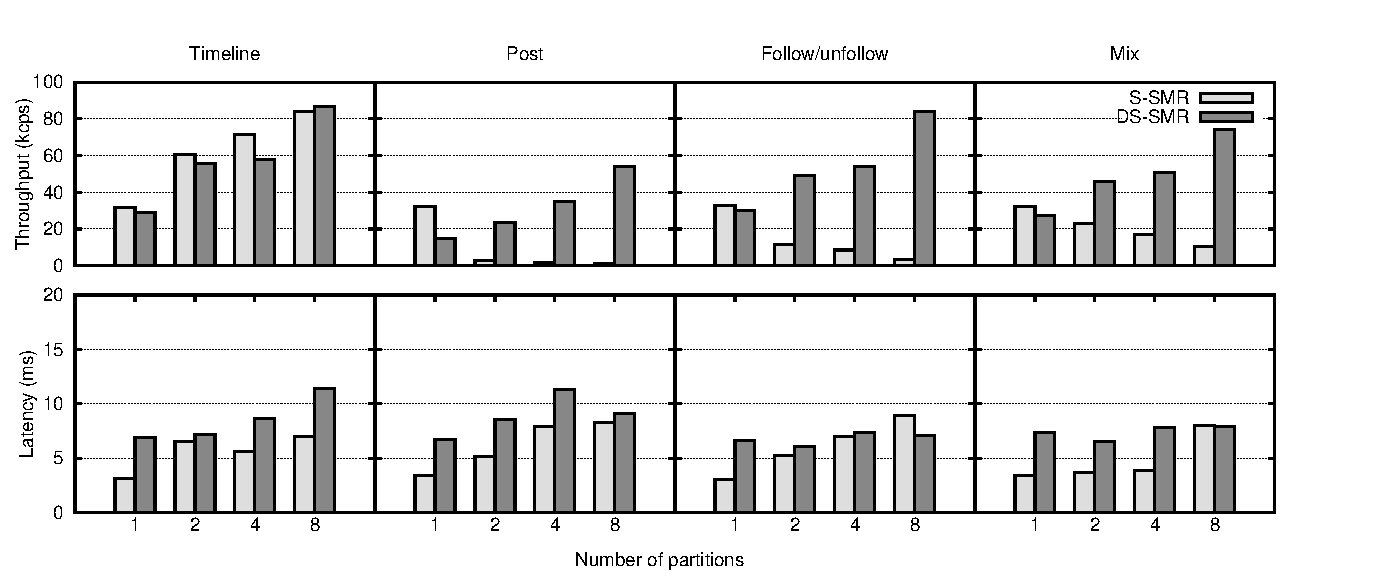
\includegraphics[width=1\linewidth]{figures/experiments/dssmr/strong-locality}
% \end{minipage}
% \caption{Results of \dssmrappname\ running with \ssmr\ and \dssmr{} with strong-locality workload. Throughput is shown in thousands of commands per second (kcps).}
% \label{fig:dssmr-strongloc}
% \end{figure*}


% \begin{figure*}[ht!]
% \begin{minipage}[b]{1\linewidth}
% \centering
%       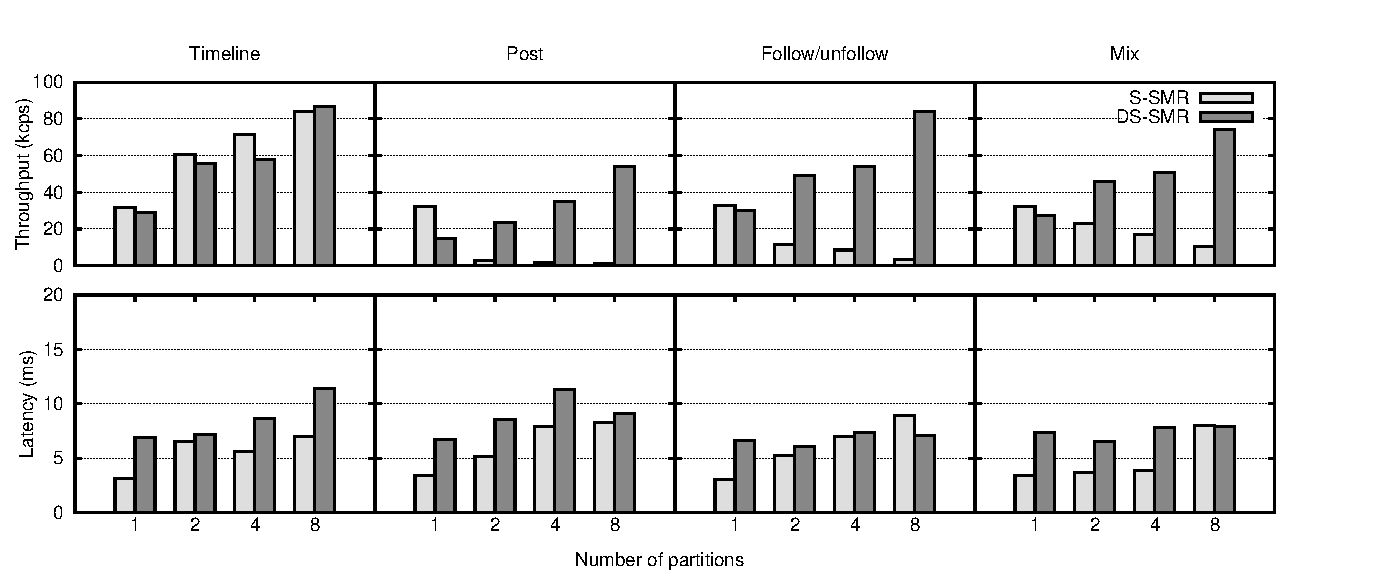
\includegraphics[width=1\linewidth]{figures/experiments/dssmr/weak-locality}
% \end{minipage}
% \caption{Results of \dssmrappname\ running with \ssmr\ and \dssmr{} with weak-locality workload. Throughput is shown in thousands of commands per second (kcps).}
% \label{fig:dssmr-weakloc}
% \end{figure*}

\begin{figure*}[ht!]
\centering
\begin{subfigure}{1\columnwidth}
      \centering
      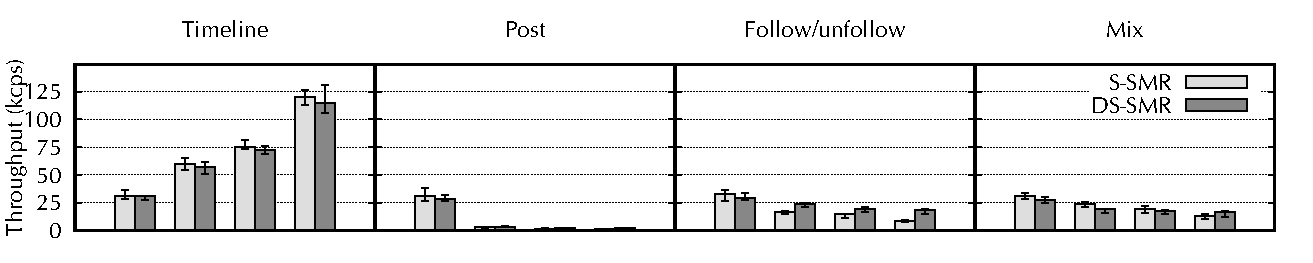
\includegraphics[width=\textwidth]{./figures/experiments/dssmr/dssmr-weak-locality-tp}
\end{subfigure}
\begin{subfigure}{1\columnwidth}
      \centering
      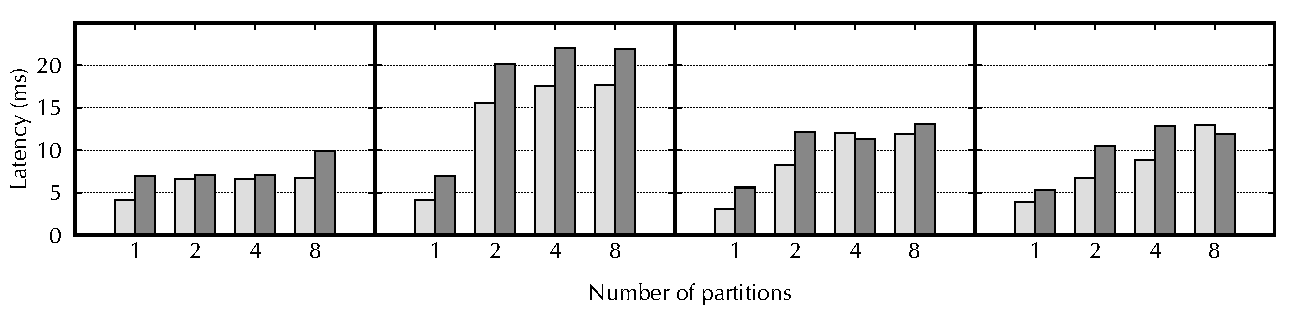
\includegraphics[width=\textwidth]{./figures/experiments/dssmr/dssmr-weak-locality-lat}
\end{subfigure}
\caption{Results of \dssmrappname\ running with \ssmr\ and \dssmr{} with weak-locality workload. Throughput is shown in thousands of commands per second (kcps).}
\label{fig:dssmr-weakloc}
\end{figure*}

\subsection{Environment setup and configuration parameters}
\label{sec:dssmr-evaluation:setup}

We conducted all experiments on a cluster that had two types of nodes: (a) HP
SE1102 nodes, equipped with two Intel Xeon L5420 processors running at 2.5 GHz
and with 8 GB of main memory, and (b) Dell SC1435 nodes, equipped with two AMD
Opteron 2212 processors running at 2.0 GHz and with 4 GB of main memory. The HP
nodes were connected to an HP ProCurve 2920-48G gigabit network switch, and the
Dell nodes were connected to another, identical switch. Those switches were
interconnected by a 20 Gbps link. All nodes ran CentOS Linux 7.1 with kernel
3.10 and had the OpenJDK Runtime Environment~8 with the \mbox{64-Bit} Server VM
(build 25.45-b02).
%We kept the clocks synchronized using NTP in order to measure latency
%components involving events in different computers.

For the experiments, we use the following workloads: Timeline (composed only of
getTimeline requests), Post (only post requests), Follow/unfollow (50\% of
follow requests and 50\% of unfollow), and Mix (7.5\% post, 3.75\% follow,
3.75\% unfollow, and 85\% getTimeline).

\subsection{Results for strong locality}
\label{sec:dssmr-evaluation:strongloc}


\begin{figure*}[ht!]
\begin{minipage}[b]{1\linewidth}
\centering
      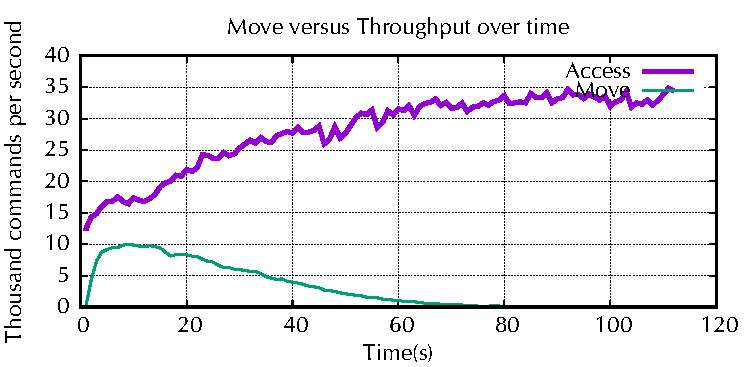
\includegraphics[width=0.6\linewidth]{figures/experiments/dssmr/move-vs-throughput}
\end{minipage}
\caption{Number of move versus throughput in DS-SMR in the experiment of Post commands on 4 partitions}
\label{fig:dssmr-move-vs-tp}
\end{figure*}

% THROUGHPUT

We can see in Figure~\ref{fig:dssmr-strongloc} and Table~\ref{tbl:results} the
results achieved with \dssmrappname{}, running with a strong-locality workload.
For the Timeline workload, the throughput with \dssmr\ and \ssmr\ are very
similar. This happens because getTimeline requests are optimized to be
single-partition: all posts in a user's timeline are stored along with the User
object. Every getTimeline requests accesses a single User object (of the user
whose timeline is being requested). This is the ideal workload for \ssmr{}. In
\dssmr{}, the partitioning does not change, and consulting the oracle becomes
unnecessary thanks to the local cache at each client. This happens because there
are no other commands in the Timeline workload.

In the Post workload, every command accesses up to all partitions in the system,
which is the worst case for \ssmr{}: the more partitions are involved in the
execution of a command, the worst is the system's performance. We can see that
the throughput of \ssmr\ decreases significantly as the number of partitions
increases. For \dssmr{}, we can see that the system throughput scales with the
number of partitions. This happens because User objects that are accessed
together but are in different partitions are moved to the same partition
based on the interests of the users. As the execution proceeds, this leads to a
lower rate of multi-partition commands, which allows throughput to scale. (In
the case of posts on 2 partitions, the number of move commands started at 3
kcps, with throughput of 23 kps, and eventually reduced to less than 0.1 kcps.)
As a result the throughput improvement of \dssmr{} with respect to \ssmr\
increases over time. With eight partitions, \dssmr{} sports a performance that
is 45 times that of \ssmr!

With the Follow/unfollow workload, the system performs in a similar way to that
observed with the Post workload. The difference is that each follow or unfollow
request accesses only two User objects, whereas every post request may affect an
unbounded number of users. For this reason, each follow/unfollow command is
executed at most by two partitions in \ssmr{}. In \dssmr{}, a single move
command is enough to have all User objects affected by such a command in the
same partition. For this reason, both replication techniques have better
throughput under the Follow/unfollow workload than with Post. As with the Post
workload, \dssmr{}'s advantage over \ssmr\ increases with the number of
partitions, reaching up to almost 25 times with eight partitions.

We approximate a realistic distribution of commands with the Mix workload. With
such a workload, \ssmr\ does not perform as bad as in the Post or
Follow/unfollow workloads, but the system throughput still decreases as
partitions are added. As with the other workloads, \dssmr\ scaled under the Mix
workload. With eight partitions, it reached 74~kcps (thousands of commands per
second), fairly close to the ideal case (the Timeline workload), where \dssmr\
reached 86~kcps. Under the Mix workload, \ssmr\ had less than 33~kcps in the
best case (one partition) and around 10~kcps with eight partitions. In the
configuration with eight partitions, \dssmr\ reaches almost seven times \ssmr's
throughput.

Latency values with \dssmr\ are higher than with \ssmr{}. This was expected for
two reasons. First, there is an extra group of servers (the oracle) to
communicate with. Second, executing a command often means moving all accessed
objects to the same partition. Taking this into account, we consider the (often
slight) increase in latency observed with \dssmr\ a low price to pay for the
significant increase in throughput and the scalability that \dssmr\ brought to
the system; with \ssmr{}, the system did not scale with multi-partition
commands.


\begin{figure*}[ht!]
\centering
\begin{subfigure}{.48\textwidth}
      \centering
      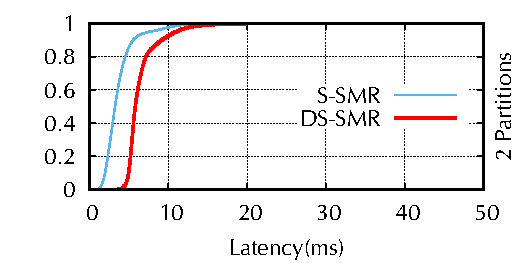
\includegraphics[width=\textwidth]{./figures/experiments/dssmr/latency-cdf-mix-2p}
\end{subfigure}
\begin{subfigure}{.48\textwidth}
      \centering
      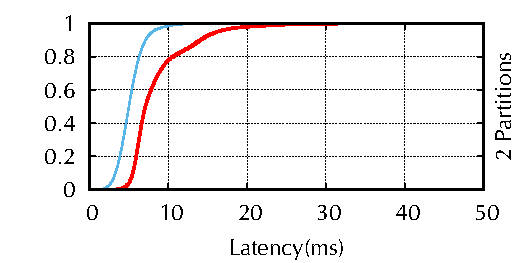
\includegraphics[width=\textwidth]{./figures/experiments/dssmr/latency-cdf-post-2p}
\end{subfigure}
\begin{subfigure}{.48\textwidth}
      \centering
      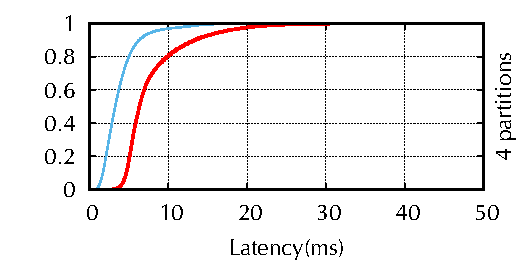
\includegraphics[width=\textwidth]{./figures/experiments/dssmr/latency-cdf-mix-4p}
\end{subfigure}
\begin{subfigure}{.48\textwidth}
      \centering
      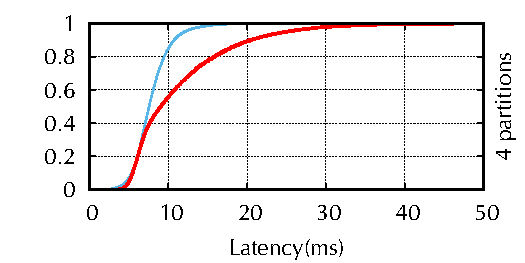
\includegraphics[width=\textwidth]{./figures/experiments/dssmr/latency-cdf-post-4p}
\end{subfigure}
\begin{subfigure}{.48\textwidth}
      \centering
      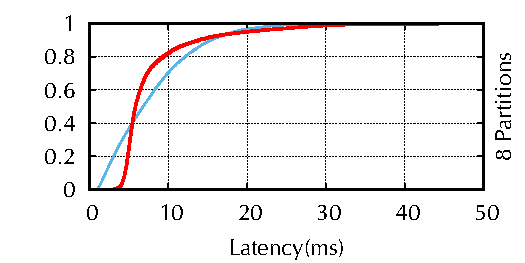
\includegraphics[width=\textwidth]{./figures/experiments/dssmr/latency-cdf-mix-8p}
      \caption{Mix}
\end{subfigure}
\begin{subfigure}{.48\textwidth}
      \centering
      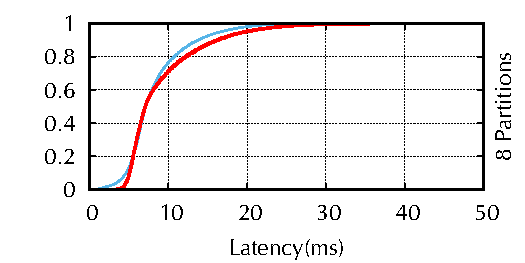
\includegraphics[width=\textwidth]{./figures/experiments/dssmr/latency-cdf-post-8p}
      \caption{Post}
\end{subfigure}
\caption{Cumulative distribution function (CDF) of latency for mix workloads of \dssmr\ and \ssmr.}%
\label{fig:dssmr-cdf}
\end{figure*}


\begin{table*}[htp]
      \vspace{10mm}
      \caption{Absolute values of \dssmrappname\ running \ssmr\ and \dssmr{}.}
      \centering
      \begin{adjustbox}{max width=\textwidth}
      \begin{tabular}{|l|c|c|c|c|c|c|c|c|c|c|c|c|c|c|c|c|} \hline
               & \multicolumn{4}{|c|}{Timeline}  &  \multicolumn{4}{|c|}{Post}   &  \multicolumn{4}{|c|}{Follow/unfollow}  &  \multicolumn{4}{|c|}{Mix}    \\ \hline
               & 1     & 2     & 4     & 8       & 1     & 2     & 4   & 8    & 1     & 2     & 4       & 8           & 1     & 2     & 4     & 8     \\ \hline\hline
               & \multicolumn{16}{|c|}{Throughput (commands per second)} \\ \hline
      \ssmr\   & 32561 & 61220 & 75812 & 11867   & 32483 & 2893  & 1882  & 1190  & 32541 & 11476 & 8580    & 3371          & 32151 & 22803 & 16822 & 10657 \\ \hline
      \dssmr\  & 29248 & 56347 & 70717 & 11175   & 19248 & 23667 & 35547 & 54025 & 30215 & 48976 & 54025   & 83880         & 27101 & 45686 & 50671 & 74257 \\ \hline\hline
               & \multicolumn{16}{|c|}{\textbf{Throughput rate = \dssmr\ tput / \ssmr\ tput}} \\ \hline
               & \textbf{0.91} & \textbf{0.92}  & \textbf{0.81} & \textbf{1.03}     & \textbf{0.46}   & \textbf{8.08}   & \textbf{18.48}  & \textbf{45.00} & \textbf{0.93} & \textbf{4.27} & \textbf{6.30} & \textbf{24.88} & \textbf{0.84} & \textbf{2.00} & \textbf{3.01} & \textbf{6.97} \\ \hline\hline
               & \multicolumn{16}{|c|}{Latency (milliseconds)} \\ \hline
      \ssmr\   & 3.1 & 6.6 & 5.6 & 7.0  & 3.4 & 5.2  & 7.9  & 8.3  & 3.0  & 5.2  & 7.0  & 8.8  & 3.4  & 3.7  & 3.8  & 7.9  \\ \hline
      \dssmr\  & 6.9 & 7.1 & 8.6 & 11.4 & 6.7 & 8.6  & 11.3 & 9.1  & 6.6  & 6.1  & 7.4  & 7.0  & 7.3  & 6.5  & 7.8  & 7.9  \\ \hline
      \end{tabular}
      \end{adjustbox}
      \label{tbl:results}
      \vspace{10mm}
\end{table*}%


\subsection{Results for weak locality} \label{sec:dssmr-evaluation:weakloc}

The Figure~\ref{fig:dssmr-weakloc} shows the results achieved with
\dssmrappname{}, running with a weak-locality workload.

\fxnote{Add few more words on this performance. [Should we include this here?]}

\section{Conclusion}
\label{sec:dssmr-conclusion}
This chapter introduced \dssmr, the initial idea of \dynastar. So far, we have
proposed an approach that allows scaling state machine replication by
dynamically repartitioning application state based on the workload.  Variables
that are usually accessed together are moved to the same partition, which
significantly improves scalability. However, in order to reduce the chances of
skewed load among partitions in \dssmr\, the destination partition is chosen
randomly. Although this heuristic algorithm could bring a balanced partitioning,
it fails to guarantee optimal partitioning and to minimize the rate of
multi-partition commands. In the next chapter, we will discuss more details
about reaching an optimized partitioning.



\chapter[Optimized partitioning for SMR]{Optimized partitioning for SMR}
\label{sec:dynastar}


\dssmr{} addresses the limitations of \ssmr{} by adapting the partitioning
scheme as workloads change, by moving data ``on demand'' to maximize the number
of single-partition user commands, while avoiding imbalances in the load of the
partitions. The major challenge in this approach is determining how the system
selects the partition to which to move data. \dssmr{} selects partitions
randomly, which allows for a completely decentralized implementation, in which
partitions make only local choices about data movement. We refer to this
approach as \emph{decentralized partitioning}. This approach works well for data
with \emph{strong locality}, but it is unstable for workloads with \emph{weak
locality}.\footnote{Workloads are referred as \emph{strong locality} if that can
be partitioned in a way that would both (i) allow commands to be executed at a
single partition only, and (ii) evenly distribute data so that load is balanced
among partitions. Conversely, workloads that cannot avoid multi-partition
commands with balanced load among partitions exhibit \emph{weak locality}.}
This happens because with weak locality, objects in \dssmr{} are constantly
being moved back and forth between partitions without converging to a stable
configuration.

In this chapter, we introduce \dynastar, a new dynamic approach to the state
partitioning problem. Like the other dynamic approach, \dynastar does not
require any a priori knowledge about the workload. However, \dynastar differs
from the prior approach because it maintains a location oracle with a global
view of the application state. The oracle minimizes the number of state
relocations by monitoring the workload, and re-computing an optimized
partitioning on demand using a static partitioning algorithm.

The location oracle maintains two data structures: (i) a mapping of application
state variables to partitions, and (ii) a \emph{workload graph} with state
variables as vertices and edges as commands that access the variables. Before a
client submits a command, it contacts the location oracle to discover the
partitions on which state variables are stored.  If the command accesses
variables in multiple partitions, the oracle chooses one partition to execute
the command and instructs the other involved partitions to temporarily relocate
the needed variables to the chosen partition. Of course, when relocating a
variable, the oracle is faced with a choice of which partition to use as a
destination. \dynastar chooses the partition for relocation by partitioning the
workload graph using the METIS~\cite{Abou-Rjeili:2006} partitioner and selecting
the partition that would minimize the number of state relocations.
% Although METIS does not necessarily produce the best possible partitioning of the workload graph, it offers a good compromise between performance and partitioning quality.

To tolerate failures, \dynastar implements the oracle as a regular partition,
replicated in a set of nodes. To ensure that the oracle does not become a
performance bottleneck, clients cache location information. Therefore, clients
only query the oracle when they access a variable for the first time or when
cached entries become invalid (i.e., because a variable changed location).
\dynastar copes with commands addressed to wrong partitions by telling clients
to retry a command.

We implemented \dynastar and compared its performance to other schemes,
including an idealized approach that knows the workload ahead of time. Although
this scheme is not achievable in practice, it provides an interesting baseline
to compare against. \dynastar's performance rivals that of the idealized scheme,
while having no a priori knowledge of the workload. We show that \dynastar
largely outperforms existing dynamic schemes under two representative workloads,
the TPC-C benchmark and a social network service. We also show that the location
oracle never becomes a bottleneck and can handle workload graphs with millions
of vertices.

In summary, this chapter makes the following contributions:
\begin{itemize}
\item It introduces \dynastar and discusses its implementation.
\item It evaluates different partitioning schemes for state machine replication
under a variety of conditions.
\item It presents a detailed experimental evaluation of \dynastar using the
TPC-C benchmark and a social network service populated with a real social
network graph that contains half a million users and 14 million edges.
\end{itemize}


The rest of the chapter is structured as follows.
Section~\ref{sec:dynastar-idea} introduces \dynastar and describes the technique in detail.
Section~\ref{sec:dynastar-algo} overviews our prototype.
Section~\ref{sec:dynastar-experiments} reports on the results of our experiments.
Section~\ref{sec:dynastar-conclusion} concludes the chapter.


\section{General idea}
\label{sec:dynastar-idea}

\dynastar defines a dynamic mapping of application variables to partitions.
Application programmers may also define other granularity of data when mapping
application state to partitions. For example, in our social network application
(\S\ref{sec:imp:\dynastarappname}), each user (together with the information associated
with the user) is mapped to a partition; in our TPC-C implementation
(\S\ref{sec:imp:tpcc}), every district in a warehouse is mapped to a partition.
Such a mapping is managed by a partitioning oracle, which is handled as a
replicated partition. The oracle allows the mapping of variables to partitions
to be retrieved or changed during execution. To simplify the discussion, in
\S\ref{sec:dynastar-idea}--\ref{sec:dynastar-detailed} we initially assume
that every command involves the oracle. In \S\ref{sec:dynastar-optm}, we explain how
clients can use a cache to avoid the oracle in the execution of most commands.

Clients in \dynastar submit commands to the oracle and wait for the reply.
\dynastar\ supports three types of commands: $create(v)$ creates a new variable
$v$ and initially maps it to a partition defined by the oracle; $access(\omega)$
is an application command that reads and modifies variables in set $\omega
\subseteq \vvm$; and $delete(v)$ removes $v$ from the service state. The reply
from the oracle is called a $prophecy$, and usually consists of a set of tuples
$\langle v, \ppm \rangle$, meaning $v \in \ppm$, and a target partition $\ppm_d$
on which the command will be executed. The $prophecy$ could also tell the
clients if a command cannot be executed (e.g., it accesses variables that do not
exist). If the command can be executed, the client waits for the reply from the
target partition.

If a command $C$ accesses variables in $\omega$ on a single partition, the
oracle multicasts $C$ to that partition for execution. If the command accesses
variables on multiple partitions, the oracle multicasts a $global(\omega,\ppm_d,
C)$ command to the involved partitions to gather all variables in $\omega$ to
the target partition $\ppm_d$. After having all required variables, the target
partition executes command $C$, sends the reply to the client, and returns the
variables to their source.

The oracle also collects hints from clients and partitions to build up a
workload graph and monitors the changes in the graph.
%\dynastar models a service workload as a graph $G = (V, E)$, where
In the workload graph, vertices represent state variables and edges dependencies
between variables. An edge connects two variables in the graph if a command
accesses both of them.
%A location oracle builds the workload graph based on feedback from the clients
%or partitions, as commands are executed.
Periodically, the oracle computes a new optimized partitioning and sends the
partitioning plan to all partitions. Upon delivering the new partitioning, the
partitions exchange variables and update their state accordingly. \dynastar
relocates variables without blocking the execution of commands.


\section{Detailed Algorithm}
\label{sec:dynastar-algo}

\label{sec:dynastar-detailed}

\begin{algorithm}[h!]
%\small
\footnotesize

\begin{distribalgo}[1]

%\vspace{1.0mm}

\INDENT{\colorbox{\coloralgo}{To issue a command $C$, the client does:}}

\vspace{1.0mm}
	% \STATE $\omega \leftarrow vars(C)$
	% \COMMENT{variables accessed by $C$}

	% \IF[if $v$ $\neg$exists in cache:]{$\exists v \in \omega : cache(\{v\}) = \bot$}
		\STATE \amcast$($oracle, $exec(C))$
		% \COMMENT{multicast command to $oracle$}
		\STATE wait for $prophecy$
		\IF[if receive $nok$ then...]{$prophecy = nok$}
			\STATE $reply \leftarrow prophecy$
			\COMMENT{...there's nothing to execute}
		\ELSE[in this case, $prophecy$ is $(dest)$]
			% \STATE $cache(\{v\}) \leftarrow prophecy$
			\STATE wait for $reponse$ from a server in $prophecy$
			\STATE $reply \leftarrow reponse$
		\ENDIF
	% \ELSE[if all vars in $\omega$ exist in cache]
	% 	\STATE $\ppm_d \leftarrow target(G_W, \omega)$
	% 	\COMMENT{select partition to execute}
	% 	\STATE \amcast$(\ppm_d, exec(C))$
	% 	\STATE wait for $reponse$ from server $\ppm_d$
	% 	\IF[if receive $retry$ then...]{$reponse = retry$}
	% 		\STATE $cache(\{v\}) \leftarrow \bot$
	% 		\COMMENT {clear cache of $\omega$}
	% 		\STATE return retry $C$
	% 	\ELSE
	% 		\STATE $reply \leftarrow reponse$
	% 	\ENDIF	

	% \ENDIF
\STATE return $reply$ to the application

\vspace{1.0mm}

% \INDENT{\colorbox{\coloralgo}{\textbf{function} cache$(vars)$}}
% 	\STATE $dests \leftarrow \{ \ppm : \exists v \in vars \cap \ppm \}$
% 	\STATE return $dests$
% \ENDINDENT

% \vspace{1.0mm}
% \INDENT{\colorbox{\coloralgo}{\textbf{function} target$(vars)$}}
% 	\STATE $\ppm \leftarrow$ compute destination partition for $vars$ from\\ \hspace{8mm}current $\ppm_1, ..., \ppm_m$ and $\ip_1, ..., \ip_m$ partitioning
% 	\STATE return $\ppm$
% \ENDINDENT	

\ENDINDENT

\caption{Client}
\label{alg:client_proxy}
\end{distribalgo}
\end{algorithm}
% \fxnote{Fixing some notation of algorithm}
\begin{algorithm}[htbp!]
%\small
\footnotesize

\begin{distribalgo}[1]

%\vspace{1.0mm}
\INDENT{\emph{Initialization:}}
	\STATE $changes \leftarrow 0$
	\STATE $\vvm \leftarrow \emptyset$
	\STATE $\llm=\{ \ppm=\{v:v \in \vvm\} : \ppm \in \{\ppm_1,...,\ppm_k\} \} \leftarrow \emptyset$
\ENDINDENT

\INDENT[\textbf{Task 1}]{\colorbox{\coloralgo}{\textbf{when} \amdel$(exec(C))$}}
	\INDENT{\textbf{case} $C$ is a $create(v)$ command:}
		\IF[if $v$ already exists...]{$\parts(\{v\}) \neq \bot$}
			\STATE $prophecy \leftarrow nok$
			\COMMENT{...notify client}
		\ELSE[if $v$ doesn't exist...]
			\STATE $\ppm \leftarrow$ choose $v$'s partition
			% \COMMENT{...determine $v$'s partition}
			\STATE $prophecy \leftarrow \ppm$
			\COMMENT{prepare client's response}
			% \STATE $alldest \leftarrow \{oracle\} \cup \{ \ppm \}$
			\STATE \amcast$(\{oracle, \ppm\}, \langle\ppm,create(v)\rangle)$
%					\COMMENT{send command to partition}
		\ENDIF
	\ENDINDENT

	\INDENT{\textbf{case} $C$ is any command, but $create(v)$:}
		\STATE $\omega \leftarrow vars(C)$
		\COMMENT{variables accessed by $C$}
		\IF[if $v$ $\neg$exists:]{$\exists v \in \omega : \parts(\{v\}) = \bot$}
			\STATE $prophecy \leftarrow nok$
			\COMMENT{tell the client}
		\ELSE[if all vars in $\omega$ exist]
			\STATE $dests \leftarrow \parts(\omega)$
			\COMMENT{get all partition involved}
			\STATE $\ppm_d \leftarrow target(dests, C)$
			\COMMENT{$\ppm_d$ will excecute $C$}
			\STATE \amcast$(dests, C)$
			\STATE $prophecy \leftarrow \ppm_d$
		\ENDIF
	\ENDINDENT
	\STATE send $prophecy$ to the client
\ENDINDENT
\vspace{1.0mm}

\INDENT[\textbf{Task 2}]{\colorbox{\coloralgo}{\textbf{when} \amdel$(\langle\ppm_v,create(v)\rangle)$}}
%	\INDENT{\textbf{case} $C$ is a $create(v)$ command:}
%	\STATE \rmcast$(\ppm_v, \langle signal, C \rangle )$
	% \STATE $\forall x \in \ppm_v$: \rmcast$(x, \langle signal, create(v) \rangle)$
	\STATE \rmcast$(\{\ppm_v, oracle\}, \langle signal, create(v) \rangle)$
	\COMMENT{exchange signal...}
	\STATE wait until $\langle signal, create(v) \rangle \in rcvd\_msgs$
	\COMMENT{...to coordinate}
	\STATE $\vvm \leftarrow \vvm \cup \{v\}$
	\STATE $\llm\{\ppm\} \leftarrow \llm\{\ppm\} \cup \{v\}$
	\COMMENT{add $v$ to service state}
% \STATE send $ok$ to the client
\ENDINDENT


\vspace{1.0mm}
\INDENT[\textbf{Task 3}]{\colorbox{\coloralgo}{\textbf{when} r-deliver $( \langle val, C \rangle )$}}
%\INDENT[\textbf{Task 3}]{\colorbox{\coloralgo}{\textbf{when} \rmdel$( \langle val, C \rangle )$}}
	\STATE $rcvd\_msgs \leftarrow rcvd\_msgs \cup \{\langle val, C \rangle\}$
\ENDINDENT

\vspace{1.0mm}

\INDENT[\textbf{Task 4}]{\colorbox{\coloralgo}{\textbf{when} \amdel$(hint(V_h,E_h))$}}
	\STATE update $G_W$ with $(V_h,E_h)$
	\STATE $changes \leftarrow changes + 1$
	\COMMENT{increase number of changes in graph}
	\IF {$changes \geq threshold$}
		\STATE $\llm_{optimized}  \leftarrow$ compute $\{\ppm=\{v:v \in \vvm\} : \ppm \in \{\ppm_1,...,\ppm_k\}\}$ from $G_W$
		% \STATE $alldest \leftarrow \{oracle\} \cup all partitions$
		\STATE \amcast$(\{oracle, all\_partitions\}, (\llm_{optimized}))$
		\STATE $changes \leftarrow 0$
	\ENDIF
\ENDINDENT

\vspace{1.0mm}

\INDENT[\textbf{Task 5}]{\colorbox{\coloralgo}{\textbf{when} \amdel$(\mathit{\llm_{optimized}})$}}
	\STATE $\llm \leftarrow \llm_{optimized}$
\ENDINDENT

\vspace{1.5mm}

\textbf{Algorithm variables:}

\vspace{1mm}

$G_W$: the graph represent the service state

$changes$: number of changes in the graph

% $partitioning$: the partition configuration of $G_W$

$\vvm$: the service state

$\llm$: the location mapping of state variables


\caption{Oracle}
\label{alg:dynastar-oracle_proxy}
\end{distribalgo}
\end{algorithm}




\begin{algorithm}[h!]
%\small
\footnotesize

\begin{distribalgo}[1]

\INDENT[\textbf{Task 1}]{\colorbox{\coloralgo}{\textbf{when} \amdel$(C)$}}
	\STATE $\omega \leftarrow vars(C)$
	\COMMENT{variables accessed by $C$}
	\IF[\textbf{Task 1a}]{$\omega \subseteq \ppm$}
		\STATE execute command $C$
		\STATE send response to the client
	\ELSE[\textbf{Task 1b}]
		\STATE $dests \leftarrow \parts(\omega)$
		\COMMENT{get all involved partition}
		\STATE $\ppm_d \leftarrow target(dests, C)$
		\COMMENT{$\ppm_d$ $\in dest$ will execute $C$}
		\STATE $\ppm_s \leftarrow dests \setminus \ppm_d$
		\COMMENT{$\ppm_s$ $\in dests$ will send variables}

		\IF[$\ppm$ is the target partition:] {$\ppm = \ppm_d$}
			\STATE wait until $\forall v \in \omega \setminus \ppm: \exists \langle vars, C \rangle \in rcvd\_msgs :v \in vars$
			% \STATE wait until $\omega \setminus \ppm \subseteq \bigcup \{ vars | \langle vars, C \rangle \in rcvd\_msgs \}$
			\COMMENT{wait for needed variables}
			\STATE execute command $C$
			\STATE send response to the client
			% \STATE \textbf{for} each $\pqm \in \ppm_s$ \textbf{do} $\forall x \in \pqm$: \\
			\STATE \rmcast$(\ppm_i \in \ppm_s, \langle vars, C\rangle)$
			\COMMENT{return the variables}
		\ELSE[if $\ppm$ is not the target partition:]
			\STATE $vars \leftarrow \omega \cap \ppm$
			\COMMENT{all needed variables in $\ppm$}
			\STATE \rmcast$(\ppm_d, \langle vars, C \rangle)$
			\COMMENT{send variables}
			% \STATE wait until $\forall v \in vars \in rcvd\_msgs : v \in vars$
			\STATE wait until $\langle vars, C \rangle \in rcvd\_msgs$
		\ENDIF
	\ENDIF
\ENDINDENT

\vspace{1.0mm}

\vspace{1.0mm}
\INDENT[\textbf{Task 2}]{\colorbox{\coloralgo}{\textbf{when} \amdel$(\langle\ppm, create(v)\rangle)$}}
	\STATE $\forall x \in oracle$: send $(\langle signal, create(v) \rangle )$ to $x$
	\COMMENT{exchange signal}
	\STATE wait until $\langle signal, create(v) \rangle \in rcvd\_msgs$
	\COMMENT{...coordinate}
	\STATE $\ppm \leftarrow \ppm \cup \{v\}$
	\STATE send $ok$ to the client
\ENDINDENT

\vspace{1.0mm}
\INDENT[\textbf{Task 3}]{\colorbox{\coloralgo}{\textbf{when} \amdel$(partitioning)$}}
	\STATE \textbf{for} each $\pqm \in \ppm_v \in partitioning$ \textbf{do}
	% \INDENT
		\IF{$\ppm$ is $\pqm$}
			\STATE $vars \leftarrow partitioning(\pqm) \setminus v:v \in \ppm$
			\IF {$\forall v \in var, \ppm_i \in partitioning:$ \\ \hfill $\exists \langle vars, \ppm_i \rangle \in rcvd\_msgs :v \in vars$}
				\STATE apply $partitioning$
			\ENDIF
		\ELSE
			% \rmcast$(\pqm, v:v \in \pqm, C)$
			\STATE $vars \leftarrow partitioning(\pqm) \cap v:v \in \ppm$
			\STATE $\forall\,x\!\in\!\pqm$: send$(\langle vars, \ppm \rangle )$ to $x$
			\COMMENT{send objs in $\pqm$}
		\ENDIF
	% \ENDINDENT
\ENDINDENT

\vspace{1.0mm}
\INDENT[\textbf{Task 4}]{\colorbox{\coloralgo}{\textbf{when}  r-deliver $(\langle val, C \rangle)$}}
    \STATE $rcvd\_msgs \leftarrow rcvd\_msgs \cup \{\langle val, C \rangle\}$
\ENDINDENT

\vspace{1.5mm}

\textbf{Algorithm variables:}

\vspace{1mm}

$partitioning$: the partition configuration from the $oracle$


% \vspace{1.0mm}
% \INDENT{\colorbox{\coloralgo}{\textbf{function} hint$(vars)$}}
% 	\STATE $e \leftarrow \{u, v: u,v \in vars, u \neq v\}$
% 	\STATE \rmcast(oracle, $e$)
% \ENDINDENT

\caption{Server in partition $\ppm$}
\label{alg:dynastar-server_proxy}
\end{distribalgo}
\end{algorithm}

\begin{algorithm}[h!]
  %\small
  \footnotesize

  \begin{distribalgo}[1]
  \INDENT{\colorbox{\coloralgo}{\textbf{function} target$(\ppm, C)$}}
    \STATE $\ppm_d \leftarrow$ deterministically compute partition to execute\\ \hspace{8mm} command $C$ from $\forall \ppm_i \in \ppm$
    \STATE return $\ppm_d$
  \ENDINDENT


  \vspace{1.0mm}
  \INDENT{\colorbox{\coloralgo}{\textbf{function} \parts$(vars)$}}
    \STATE $dests \leftarrow \{ \ppm : \exists v \in vars \cap \ppm \}$
    \COMMENT{get all involved partitions}
    \STATE return $dests$
  \ENDINDENT

  \vspace{1.5mm}

  % \vspace{1.0mm}
  % \INDENT{\colorbox{\coloralgo}{\textbf{function} hint$(vars)$}}
  % 	\STATE $e \leftarrow \{u, v: u,v \in vars, u \neq v\}$
  % 	\STATE \rmcast(oracle, $e$)
  % \ENDINDENT

  \caption{Shared functions of the oracle and servers $\ppm$}
  \label{alg:dynastar-share_algo}
  \end{distribalgo}
  \end{algorithm}


Algorithms~\ref{alg:dynastar-client_proxy}, \ref{alg:dynastar-oracle_proxy}, and
\ref{alg:dynastar-server_proxy} describe the client, oracle, and server processes,
respectively. We omit the delete command since the coordination involved in the
create and delete commands are analogous.

\subsubsection{The client process}

To execute a command $C$, the client atomically multicasts $C$ to the oracle
(Algorithm \ref{alg:dynastar-client_proxy}). The oracle replies with a prophecy,
which may already tell the client that $C$ cannot be executed (e.g., it needs a
variable that does not exist, it tries to create a variable that already
exists). If $C$ can be executed, the client receives a prophecy containing the
partition where $C$ will be executed. The client then waits for the result of
the execution of $C$.

\subsubsection{The oracle}

When the oracle delivers a request, it distinguishes between two cases (Task 1
in Algorithm~\ref{alg:dynastar-oracle_proxy}).
\begin{itemize}
\item If the command is to create a variable $v$, and $v$ does not already
exist, the oracle chooses a random partition for $v$, multicasts the create
command to the partition and itself, and returns the partition to the client as
a prophecy (Figure~\ref{fig:oracle_repartition}).
\item If the command reads and writes existing variables, the oracle first
checks that all such variables exist. If the variables exist and they are all in
a single partition, the oracle multicasts the command to that partition for
execution. If the variables are distributed in multiple partitions, the oracle
deterministically determines the destination partition, and atomically
multicasts a command to the involved partitions so that all variables are
gathered at the destination partition. The oracle chooses as the destination
partition the partition that contains most of the variables needed by the
command. (In case of a tie, one partition is chosen deterministically, among
those that contain most variables.) Once the destination partition has received
all variables needed by the command, it executes the command and returns the
variables to their source partition.

\end{itemize}


\begin{figure*}[h!]
\begin{minipage}[b]{1\linewidth}
\centering
      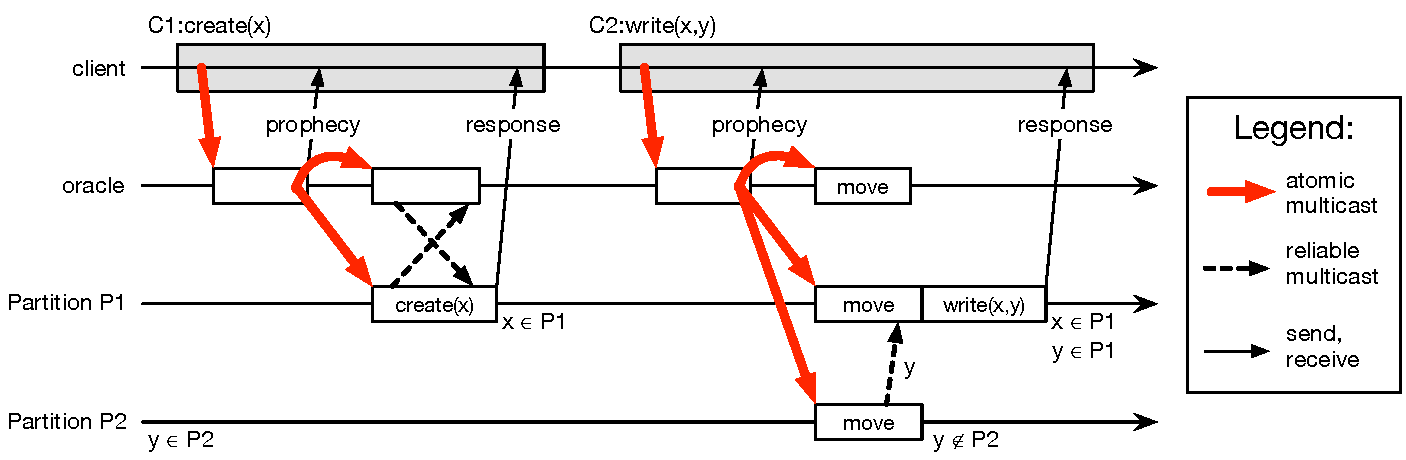
\includegraphics[width=\linewidth]{figures/dynastar}
\end{minipage}
\caption{Execution of a create (C1) and a write without client cache (C2) and with client cache (C3) in \dynastar.}
\label{fig:oracle_repartition}
\end{figure*}

Upon delivering a create (Task 2), the oracle updates its partition information.
The exchange of signals between the partition where the variable will be created
and the oracle ensures that interleaved executions between create and delete
commands will not lead to violations of linearizability (i.e., this is
essentially the execution of a multi-partition command involving the oracle and
a partition (Task 3) ~\cite{bezerra2014ssmr}). The oracle also keeps track of
the workload graph by receiving hints with variables (i.e., vertices in the
graph) and executing commands (i.e., edges in the graph). These hints can be
submitted by the clients or by the partitions, which collect data upon executing
commands and periodically inform the oracle (Task 4). The oracle computes a
partitioning plan of the graph and multicasts it to all servers and to itself.
Upon delivering a new partition plan, the oracle updates its location map
accordingly (Task 5).

To compute an optimized partitioning, the oracle uses a graph partitioner. A new
partitioning can be requested by the application, by a partition, or by the
oracle itself (e.g., upon delivering a certain number of hints). To determine
the destination partition of a set of variables, as part of a move, the oracle
uses its mapping of the current location of variables and the last computed
partitioning.

\subsubsection{The server process}

When a server delivers a command $C$, it first checks if it has all variables
needed by $C$. If the server has all such variables, it executes $C$ and sends
the response back to the client (Tasks 1a and 2 in
Algorithm~\ref{alg:dynastar-server_proxy}). If not all the variables needed by $C$ are in
that partition, the server runs a deterministic function to determine the
destination partition to execute $C$ (Task 1b). The function uses as input the
variables needed by $C$ and $C$ itself. In this case, each server that is in the
multicast group of $C$ but is not the destination partition sends all the needed
variables stored locally to the destination partition and waits to receive them
back. The destination partition waits for a message from other partitions. Once
all variables needed are available, the destination partition executes the $C$,
sends the response back to the client, and returns the variables to their
source. Periodically, the servers deliver a new partitioning plan from the
oracle (Task 3). Each server will send the variables to the designated
partition, as in the plan, and wait for variables from other partitions. Once a
server receives all variables, it updates its location map accordingly.
To determine the destination partition for a command, the servers uses the last
computed partitioning.


\section{Performance optimizations}
\label{sec:dynastar-optm}

In the algorithm presented in the previous section, clients always need to
involve the oracle, and the oracle dispatches every command to the partitions
for execution. Obviously, if every command involves the oracle, the system is
unlikely to scale, as the oracle will likely become a bottleneck. To address
this issue, clients are equipped with a location cache. Before submitting a
command to the oracle, the client checks its location cache. If the cache
contains the partition of the variables needed by the command, the client can
atomically multicast the command to the involved partition and thereby avoid
contacting the oracle.

The client still needs to contact the oracle in one of these situations: (a)~the
cache contains outdated information; or (b)~the command is a create, in
which case it must involve the oracle, as explained before. If the cache contains
outdated information, it may address a partition that does not have the
information of all the variables accessed by the command. In this case, the
addressed partition tells the client to retry the command. The client then
contacts the oracle and updates its cache with the oracle's response. Although
outdated cache information results in execution overhead, it is expected to
happen rarely since repartitioning is not frequent.

\section{Correctness}
\label{sec:dynastar-correctness}

Similar to \dssmr, we consider linearizability consistency criterion of
\dynastar. To prove that \dynastar ensures linearizability, we must show that
for any execution $\sigma$ of the system, there is a total order $\pi$ on client
commands that (i)~respects the semantics of the commands, as defined in their
sequential specifications, and (ii)~respects the real-time precedence of
commands~(\S\ref{sec:dynastar-correctness}).
%
Let $\pi$ be a total order of operations in $\sigma$ that respects $<$, the
order atomic multicast induces on commands.

To argue that $\pi$ respects the semantics of  commands, let $C_i$ be the $i$-th
command in $\pi$ and $p$ a process in partition $\ppm_p$ that executes $C_i$.
%Let $C_i$ be the $i$-th command in $\pi$ and $p$ a process in partition
%$\ppm_p$ that executes $C_i$.
We claim that when $p$ executes $C_i$, it has updated values of variables in
$vars(C_i)$, the variables accessed by $C_i$. We prove the claim by induction on
$i$. The base step trivially holds from the fact that variables are initialized
correctly. Let $v \in vars(C_i)$, $C_v$ be the last client command before $C_i$
in $\pi$ that accesses $v$, and $q$ a process in $\ppm_q$ that executes $C_v$.
From the inductive hypothesis, $q$ has an updated value of $v$ when it executes
$C_v$. There are two cases to consider: (a)~$p = q$. In this case, $p$ obviously
has an updated value of $v$ when it executes $C_i$ since no other command
accesses $v$ between $C_v$ and $C_i$. (b)~$p \neq q$. Since processes in the
same partition execute the same commands, it must be that $\ppm_p \neq \ppm_q$.
From the algorithm, when $q$ executes $C_v$, $v \in \ppm_q$ and when $p$
executes $C_i$, $v \in \ppm_p$. Thus, $q$ executed a command to move $v$ to
another partition after executing $C_v$ and $p$ executed a command to move $v$
to $\ppm_p$ before executing $C_i$. Since there is no command that accesses $v$
between $C_v$ and $C_i$ in $\pi$, $q$ has an updated $v$ when it executes $C_v$
(from inductive hypothesis), and $p$ receives the value of $v$ at $q$, it
follows that $p$ has an updated $v$ when it executes $C_i$.

% DISCLAIMER: in the proof below, I assumed a single process per partition.
% While I'm pretty sure it works for multiple processes per partition, in some
% future refinement this should be added to the proof. Also see related picture
% showing cases (a) and (b) below. Perhaps we should include such a picture too
% in a future version.
%
We now argue that there is a total order $\pi$ that respects the real-time
precedence of commands in $\sigma$. Assume $C_i$ ends before $C_j$ starts, or
more precisely, the time $C_i$ ends at a client is smaller than the time $C_j$
starts at a client, $\tec(C_i) < \tsc(C_j)$. Since the time $C_i$ ends at the
server from which the client receives the response for $C_i$ is smaller than the
time $C_i$ ends at the client, $\tes(C_i) < \tec(C_i)$, and the time $C_j$
starts at the client is smaller than the time $C_j$ starts at the first server,
$\tsc(C_j) < \tss(C_j)$, we conclude that $\tes(C_i) < \tss(C_j)$.

We must show that either $C_i < C_j$; or neither $C_i < C_j$ nor $C_j < C_i$.
For a contradiction, assume that $C_j <  C_i$ and let $C_j$ be executed by
partition $\ppm_j$.

There are two cases:
\begin{enumerate}
\item[(a)] $C_i$ is a client command executed by $\ppm_j$. In this case, since
$C_i$ only starts after $C_j$ at a server, it follows that $\tes(C_j) <
\tss(C_i)$, a contradiction.
\item[(b)] $C_i$ is a client command executed by $\ppm_i$ that first involves a
move of variables $vars$ from $\ppm_j$ to $\ppm_i$. At $\ppm_j$, $\tes(C_j) <
\tss(global(vars,\ppm_j,\ppm_i))$ since the move is only executed after $C_j$
ends. Since the move only finishes after variables in $vars$ are in $\ppm_i$ and
$C_i$ can be executed, it must be that
%\lle{move only finishes when $P_j$ gets back its variable}
$\tes(global(vars,\ppm_j,\ppm_i)) < \tss(C_i)$. We conclude that $\tes(C_j) <
\tss(C_i)$, a contradiction.
\end{enumerate}
Therefore, either $C_i < C_j$ and from the definition of $\pi$, $C_i$ precedes
$C_j$ or neither $C_i < C_j$ nor $C_j < C_i$, and there is a total order in
which $C_i$ precedes $C_j$.
%\begin{figure} \centering
%\includegraphics[width=1.2\linewidth,angle=-90]{figures/IMG_7203.JPG}
%\caption{Two cases in proof.} \end{figure}

For termination, we argue that every correct client eventually receives a
response for every command $C$ that it issues. This assumes that every partition
(including the oracle partition) is always operational, despite the failure of
some servers in the partition. For a contradiction, assume that some correct
client submits a command $C$ that is not executed. Atomic multicast ensures that
$C$ is delivered by the involved partition. Therefore, $C$ is delivered at a
partition that does not contain all the variables needed by $C$. As a
consequence, the client retries with the oracle, which moves all variables to a
single partition and requests the destination partition to execute $C$, a
contradiction that concludes our argument.



%!TEX root =  main.tex
\section{Implementation}
\label{sec:dynastar-implementation}

\subsection{Atomic multicast}

Our \dynastar prototype uses the BaseCast atomic multicast protocol
\cite{Coelho:2017}, available as open
source.\footnote{https://bitbucket.org/paulo\_coelho/libmcast} Each group of
servers in BaseCast executes an instance of
Multi-Paxos.\footnote{http://libpaxos.sourceforge.net/paxos\_projects.php\#libpaxos3}
Groups coordinate to ensure that commands multicast to multiple groups are
consistently ordered (as defined by the atomic multicast properties
\S\ref{sec:amcast}).
%Commands multicast to multiple groups coordinate to ensure that commands are
%consistently ordered (as defined by the atomic multicast properties
%\S\ref{sec:amcast}).
BaseCast is a genuine atomic multicast in that only the sender and destination
replicas of a multicast message communicate to order the multicast message.
% A genuine atomic multicast is the foundation of scalable systems, since it does
% not rely on a fixed group of processes and does not involve all processes.

\subsection{\dynastar}

Our  \dynastar prototype is written as a Java 8 library. Application designers
who use \dynastar to implement a replicated service must extend three key
classes:
 \begin{itemize}

 \item[--] \emph{PRObject}: provides a common interface for replicated data
 items. All instance of \emph{PRObject}'s sub-classes are replicated by the
 framework(i.e., objects are distributed among partitions). The application is
 agnostic to the location of those objects. \dynastar intercepts all calls to
 replicated objects and forward them to associated partition automatically.

 \item[--] \emph{ProxyClient}: provides the communication between application
 client and server, while encapsulating all complex logic of handling caches or
 retried requests. The proxy client also allows sending multiple asynchronous
 requests, and delivering corresponding response to each request.

 \item[--] \emph{PartitionStateMachine}: encapsulates the logic of the server
  proxy. The server logic is written without knowledge of the actual
  partitioning scheme. In other words, developer programs for classical state
  machine replication (i.e., full replication). The \dynastar library handles
  all communication between partitions and the oracle transparently. Objects
  that are involved in application's command will be available to the
  partition at the time it is accessed by the partitions.

 \item[--] \emph{OracleStateMachine}: computes the mapping of objects to
  partitions. The oracle can be configured to trigger repartitioning in
  different ways: repartitioning request from application, based on the number
  of changes to the graph, or based on some interval of time. Our default
  implementation uses
  METIS\footnote{http://glaros.dtc.umn.edu/gkhome/views/metis} to provide a
  partitioning based on the workload graph. While partitioning a graph, METIS
  aims to reduce the number of multi-partition commands (edge-cuts) while
  trying to keep the various partitions balanced. We configured METIS to allow
  a 20\% unbalance among partitions. METIS repartitions a graph without
  considering previous partitions. Consequently, \dynastar may need to
  relocate a large number of objects upon a repartitioning. Other partitioning
  techniques could be used to introduce incremental graph partitioning
  \cite{SerafiniTEPAS16}.
 \end{itemize}

We note one important implementation detail.  The oracle is multi-threaded: it
can serve requests while computing a new partitioning concurrently. To ensure
that all replicas start using the new partitioning consistently, the oracle
identifies each partitioning with a unique id.  When an oracle replica finishes
a repartitioning, it atomically multicasts the id of the new partitioning to
all replicas of the oracle.  The first delivered id message defines the order
of the new partitioning with respect to other oracle operations.


\subsection{TPC-C benchmark}
\label{sec:imp:tpcc}

%On average, 10\% of transactions are distributed transactions.

TPC-C is an industry standard for evaluating the performance of OLTP systems
\cite{tpcc}. TPC-C implements a wholesale supplier company. The company has a
number of distributed sales districts and associated warehouses. Each warehouse
has 10 districts. Each district services 3,000 customers. Each warehouse
maintains a stock of 100,000 items. The TPC-C database consists of 9 tables and
five transaction types that simulate a warehouse-centric order processing
application: \emph{New-Order} (45\% of transactions in the workload),
\emph{Payment} (43\%), \emph{Delivery} (4\%), \emph{Order-Status} (4\%) and
\emph{Stock-Level} (4\%).

We implemented a Java version of TPC-C that runs on top of \dynastar. Each row
in TPC-C tables is an object in \dynastar. The oracle models the workload at the
granularity of districts, thus each district and warehouse is a node in the
graph. If a transaction accesses a district and a warehouse, the oracle will
create an edge between that district and the warehouse. The objects (e.g.,
customers, orders) that belong to a district are considered part of district.
However, if a transaction requires objects from multiple districts, only those
objects will be moved on demand, rather than the whole district. The ITEM table
is replicated in all servers, since it is not updated in the benchmark. A
transaction is a set of commands that access those objects, implemented as
server procedures.

\subsection{\dynastarappname\ social network service}
\label{sec:imp:\dynastarappname}

Using \dynastar{}, we have also developed a Twitter-like social network service,
named Chirper. In our social network, users can follow, unfollow, post, or read
other users' tweets according to whom the user is following. Like Twitter, users
are constrained to posting 140-character messages.

Each user in the social network corresponds to a node in a graph. If one user
follows another, a directed edge is created from the follower to the followee.
Each user has an associated \emph{timeline}, which is a sequence of post
messages from the people that the user follows. Thus, when a user issues a post
command, it results in writing the message to the timeline of all the user's
followers.  In contrast, when users read their own timeline, they only need to
access the state associated with their own node.

Since \dynastar guarantees linearizable executions, any causal dependencies
between posts in \dynastarappname\ will be seen in the correct order. More
precisely, if user B posts a message after receiving a message posted by user A,
no user who follows A and B will see B's message before seeing A's message.

Overall, in \dynastarappname, post, follow or unfollow commands can lead to
object moves.  Follow and unfollow commands can involve at most two partitions,
while posts may require object moves from many partitions.

%Of course, other implementations are possible. But, given that users in social
%networks spend most of the time reading (i.e., performing
%getTimeline)~\cite{facebookTAO}, it is useful to implement getTimeline as an
%efficient single-partition command.


\subsection{Alternative system}

We compare \dynastar{} to an optimized version of S-SMR~\cite{bezerra2014ssmr}
and DS-SMR~\cite{le2016dssmr}, publicly
available.\footnote{https://bitbucket.org/kdubezerra/eyrie\\
https://bitbucket.org/usi-dslab/ds-smr} S-SMR scales performance with the number
of partitions under a variety of workloads. It differs from \dynastar{} in two
important aspects: multi-partition commands are executed by all involved
partitions, after the partitions exchange needed state for the execution of the
command, and S-SMR supports static state partitioning. In our experiments, we
manually optimize S-SMR's partitioning with knowledge about the workload. In the
experiments, we refer to this system and configuration as S-SMR*.
%Since all three systems (S-SMR, DS-SMR, and \dynastar) provide a common
%application-level interface, there was no additional work required to port the
%social network application.


\section{Performance evaluation}
\label{sec:dynastar-experiments}

In this section, we report results from two benchmarks: TPC-C and
\dynastarappname{} social networking service described in the previous section.
Our experiments show that \dynastar{} is able to rapidly adapt to changing
workloads, while achieving throughputs and latencies far better than the
existing state-of-the-art approaches to state machine replication partitioning.


\subsection{Experimental environment}
\label{sec:dynastar-evaluation:setup}

We conducted all experiments on Amazon EC2 T2 large instances (nodes). Each node
has 8 GB of RAM, two virtual cores and is equipped with an Amazon EBS standard
SSD with a maximal bandwidth 10000 IOPS. All nodes ran Ubuntu Server 16.04 LTS
64 and had the OpenJDK Runtime Environment~8 with the \mbox{64-Bit} Server VM
(build 25.45-b02). In all experiments, the oracle had the same resources as
every other partition: 2 replicas and 3 Paxos acceptors (in total five nodes per
partition).


\subsection{Methodology and goals}
\label{sec:dynastar-evaluation:methodology}

%In order to show the scalability of our approach we tested the performance as
%the number of partitions increases, and performance as the size and complexity
%of the graph grows.
The experiments seek to answer the following questions:
\begin{itemize}
\item \emph{What is the impact of repartitioning on a real dataset?}
\item \emph{How does partitioning affect performance when the workload grows with the number of partitions and when the workload has constant size?}
\item \emph{How does \dynastar performance compare to other approaches?}
\item \emph{How does \dynastar perform under dynamic workloads?}
\item \emph{What is the performance of the oracle?}
\end{itemize}

\paragraph*{Performance metrics.}
The latency was measured as the end-to-end time between issuing the command, and
receiving the response.  Throughput was measured as the number of posts/second
or transactions/second that the clients were able to send.

\subsection{TPC-C benchmark}
\label{sec:dynastar-evaluation:tpc-c}

In the experiments in this section, we deploy as many partitions as the number
of warehouses.

\subsubsection{The impact of graph repartitioning}
In order to assess the impact of state partitioning on performance, we ran the
TPC-C benchmark on an un-partitioned database.  Figure
~\ref{fig:tpcc_repartitioning} shows the performance of \dynastar with 8
warehouses and 8 partitions. At the first part of the experiment, all the
variables are randomly distributed across all partitions. As a result, almost
every transaction accesses all partitions. Thus, every transaction required
coordination between partitions, and objects were constantly moving back and
forth. This can be observed in the first 50 seconds of the experiment depicted
in Figure ~\ref{fig:tpcc_repartitioning}: low throughput (i.e., a few
transactions executed per second), high latency (i.e., up to several seconds),
and a high percentage of cross-partition transactions.

After 50 seconds, the oracle computed a new partitioning based on previously
executed transactions and instructed the partitions to apply the new
partitioning. When the partitions delivered the partitioning request, they
exchanged objects to achieve the new partitioning. It takes about 10 seconds for
partitions to reach the new partitioning. During the repartitioning,
transactions that access objects that are not being relocated will continue to
process. After the state is relocated, most objects involved in a transaction
can be found in a local partition, which considerably increases performance and
reduces latency.

\begin{figure}[ht!]
  \centering
    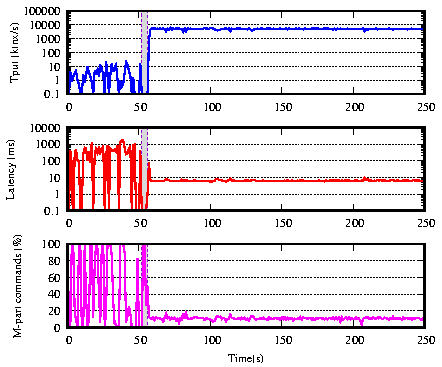
\includegraphics[width=0.8\columnwidth]{figures/experiments/dynastar/tpcc-detail-dynastar}
  \caption{Repartitioning in \dynastar; throughput (top), objects exchanged between partitions (middle),
  and percentage of multi-partition commands (bottom).}
  \label{fig:tpcc_repartitioning}
\end{figure}

\subsubsection{Scalability}
In order to show how \dynastar scales out, we varied the number of partitions
from 1 to 128 partitions. We used sufficient clients to  saturate the throughput
of the system in each experiment. Figure ~\ref{fig:tpcc_scaling} shows the peak
throughput of \dynastar and S-SMR* as we vary the number of partitions. Notice
that we increase the state size as we add partitions (i.e., there is one
warehouse per partition). The result shows that \dynastar is capable of applying
a partitioning scheme that leads to scalable performance.

\begin{figure}[ht!]
  \centering
    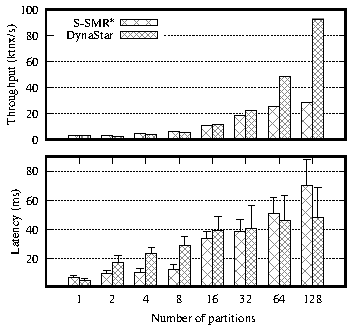
\includegraphics[width=0.7\columnwidth]{figures/experiments/dynastar/tpcc-scaling-tp-lat.pdf}
  \caption{Performance scalability with TPC-C. Throughput (in thousands of transactions per second, ktps) and latency for $\approx$75\% peak throughput in milliseconds (bars show average, whiskers show 95-th percentile).}
  \label{fig:tpcc_scaling}
\end{figure}

\subsection{Social network}

%\paragraph*{Workloads.}
We used the Higgs Twitter dataset~\cite{snapnets} as the social graph in the
experiments. The graph is a subset of the Twitter network that was built based
on the monitoring of the spreading of news on Twitter after the discovery of a
new particle with the features of the elusive Higgs boson on 4th July 2012. The
dataset consists of 456631 nodes and more than 14 million edges.
%Graphs with 0\% of edge-cuts have \emph{strong locality}.

We evaluate the performance of \dynastar and other techniques. With S-SMR*, we
used METIS to partition the data in advance. Thus, S-SMR* started with an
optimized partitioning. \dynastar started with random location of the objects.
Each client issues a sequence of commands. For each command, the client selects
a random node as the active user with Zipfian access pattern ($\rho$ = 0.95). We
focused on two types of workloads: timeline-only commands and mix commands (85\%
timeline and 15\% post). Each client operates in a closed loop, that is, the
client issues a command and then waits from the response to submit the next
command.

\begin{figure*}[ht!]
  \centering
    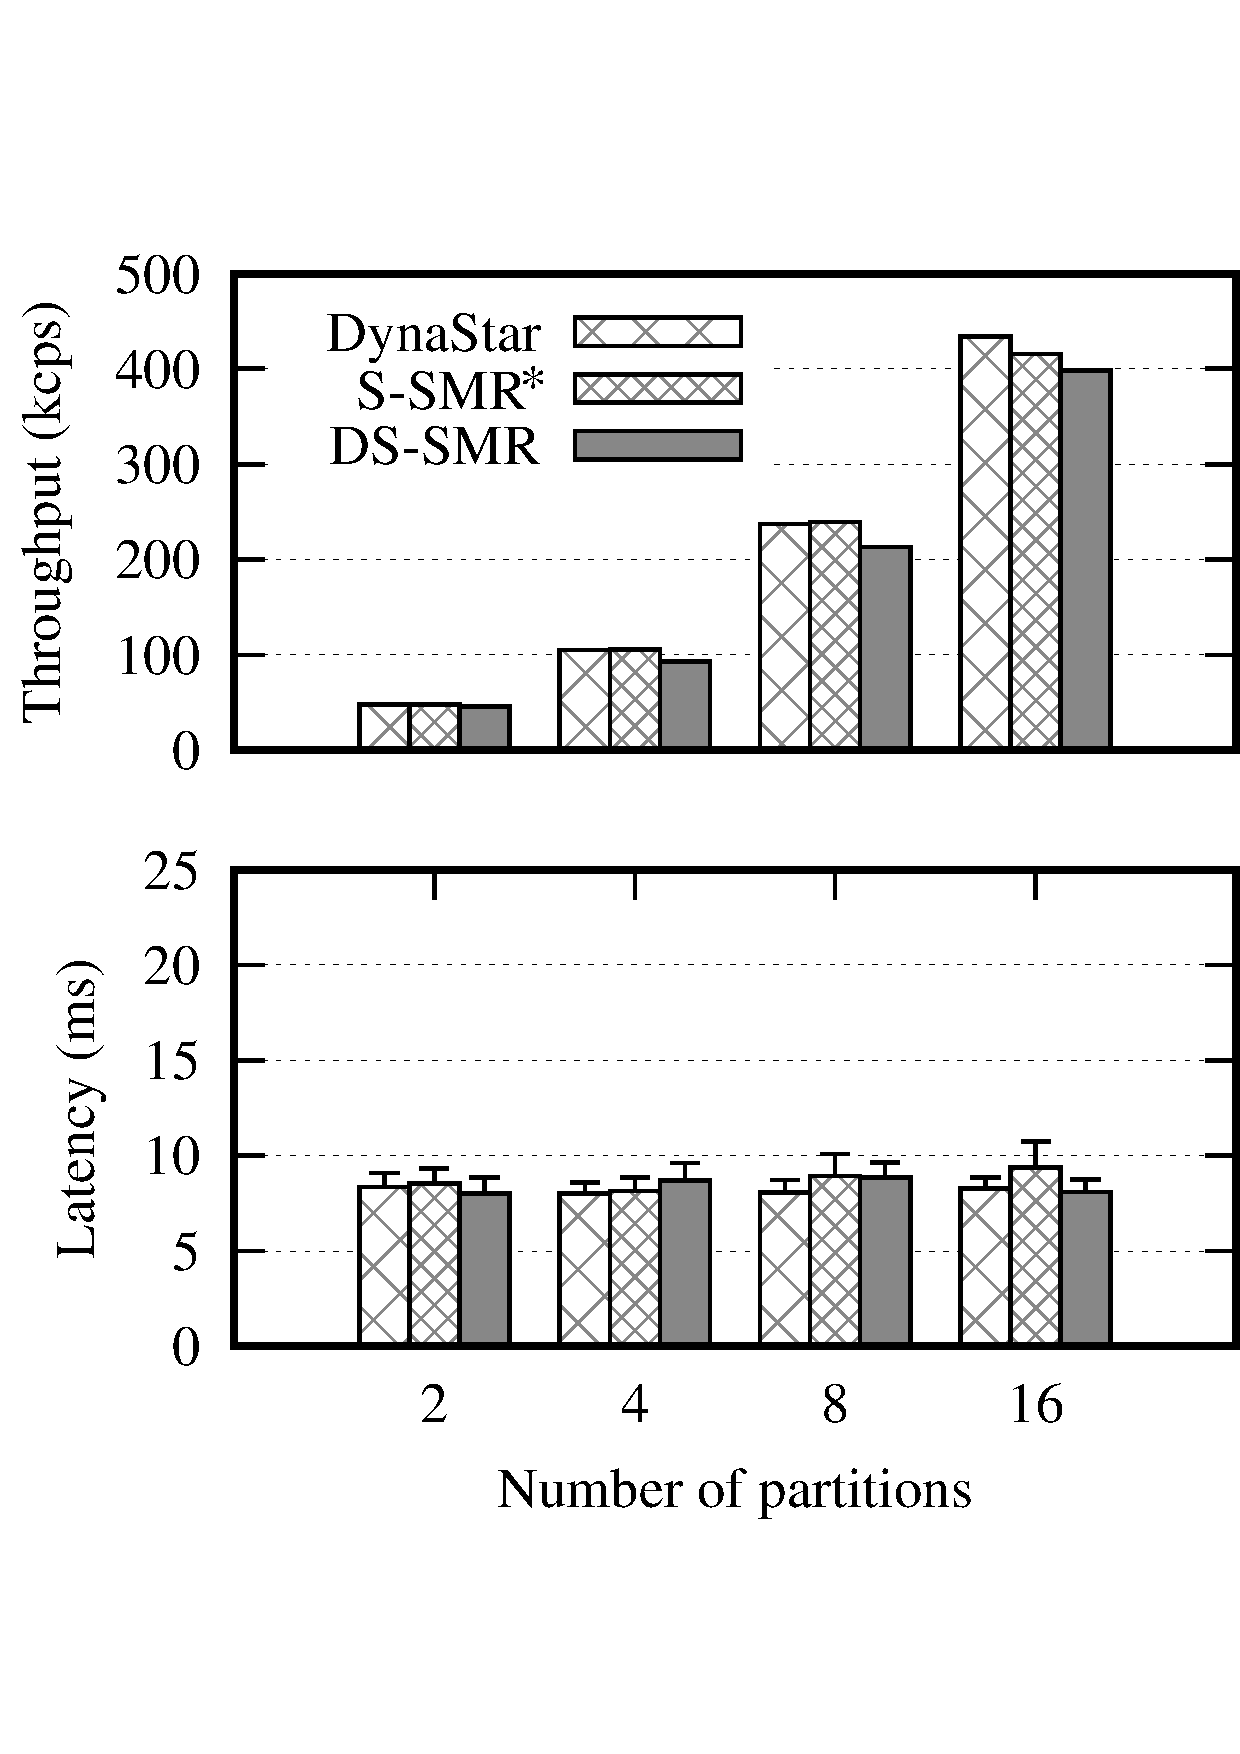
\includegraphics[width=0.6\columnwidth]{figures/experiments/dynastar/chirper-compare-timeline-no-title}
  \caption{Performance of timeline command of social network service. Throughput
  (in thousands of commands per second, kcps) and latency for different
  partitions. Latency for $\approx$75\% peak throughput in milliseconds (bars
  show average, whiskers show 95-th percentile).}
  \label{fig:socialscalability-timeline}
\end{figure*}


\begin{figure*}[ht!]
  \centering
    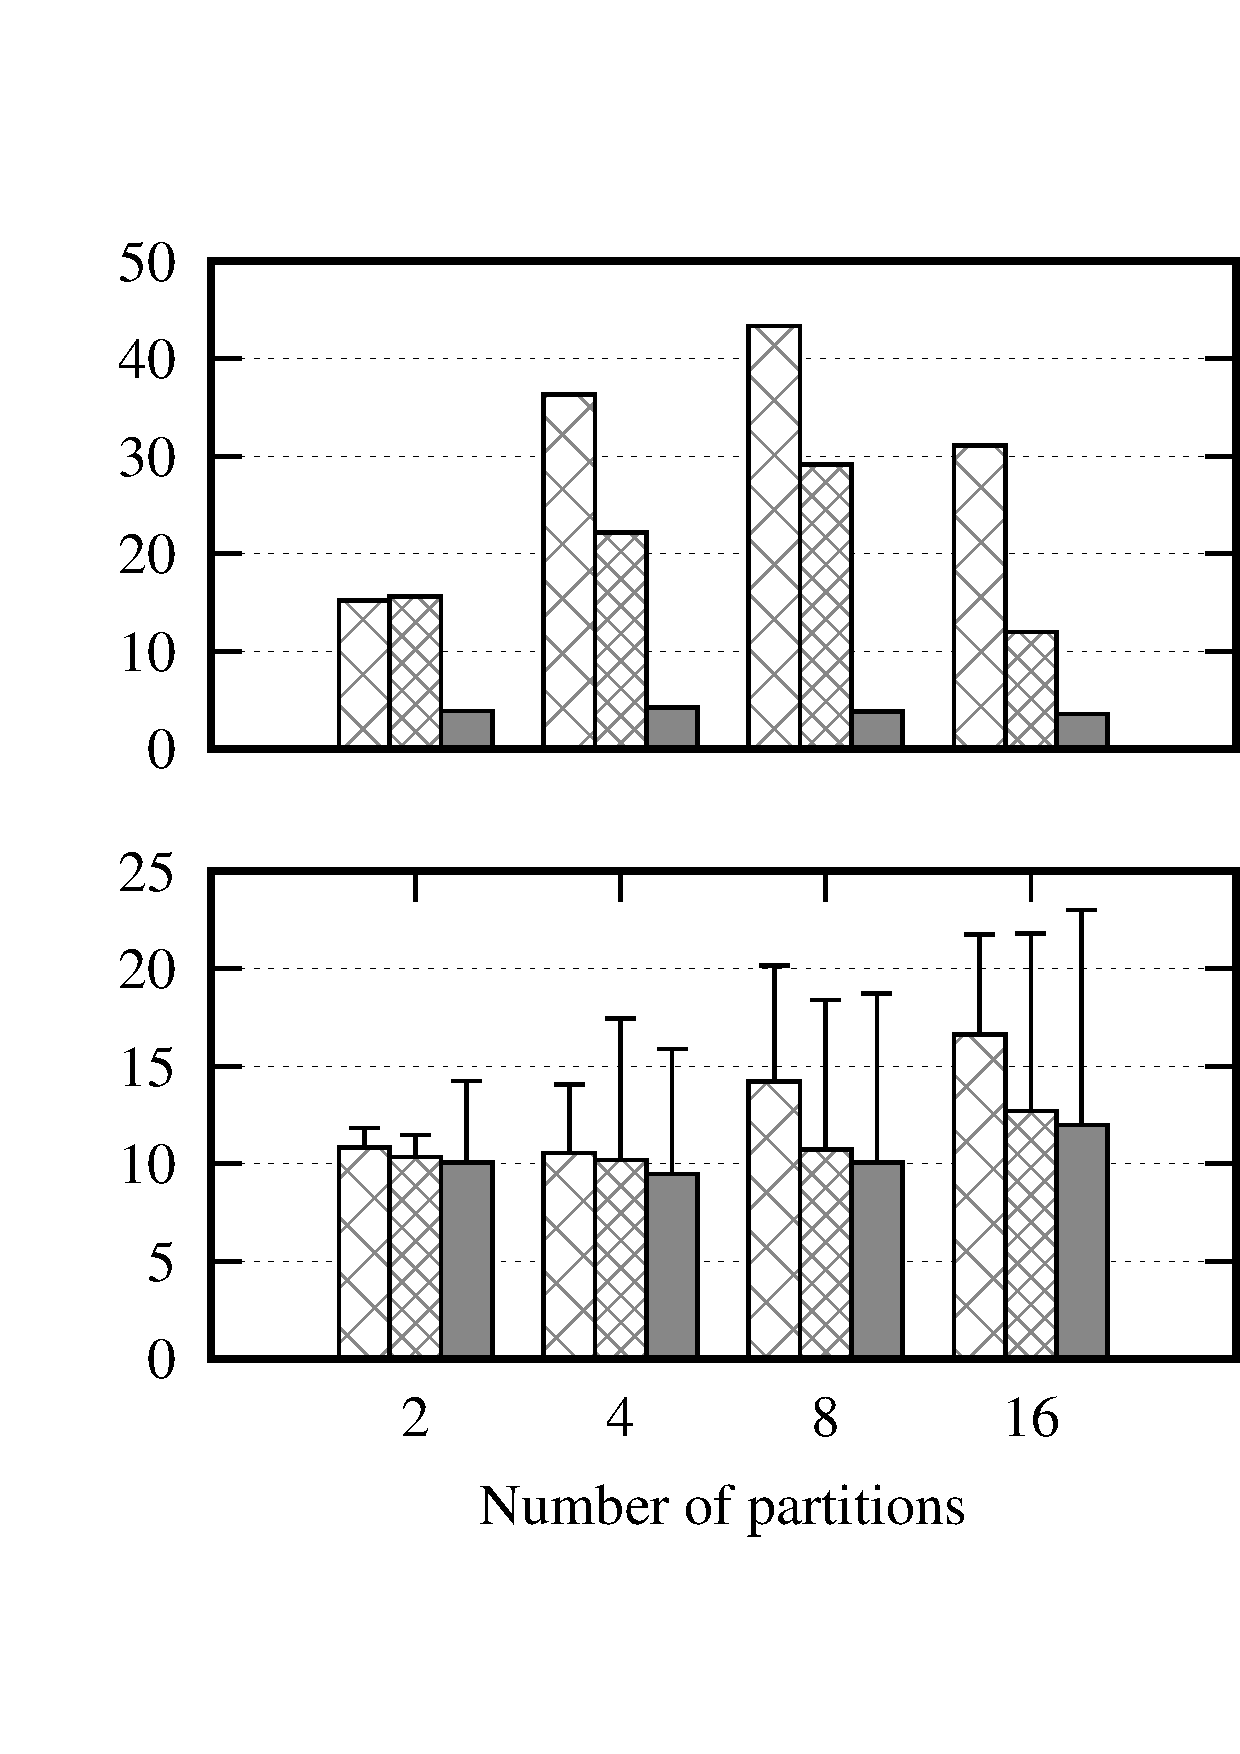
\includegraphics[width=0.6\columnwidth]{figures/experiments/dynastar/chirper-compare-mix-no-title}
  \caption{Performance of post command social network service. Throughput (in
  thousands of commands per second, kcps) and latency for different partitions.
  Latency for $\approx$75\% peak throughput in milliseconds (bars show average,
  whiskers show 95-th percentile).}
  \label{fig:socialscalability-mix}
\end{figure*}

\subsubsection{\dynastar vs. other techniques}
\label{sec:dynastar-evaluation:results}

Figure~\ref{fig:socialscalability-timeline} and~\ref{fig:socialscalability-mix}
shows the peak throughput and latency for approximately 75\% of peak throughput
(average and 95-th percentile) of the evaluated techniques as we vary the number
of partitions of the fixed graph for the social networks.

In the experiment with timeline commands, all three techniques perform
similarly. This happens because no moves occur in \dynastar or \dssmr{}, and no
synchronization among partitions is necessary for S-SMR* in this case.
Consequently, all three schemes scale remarkably well, and the difference in
throughput between each technique is due to the implementation of each one.
%Although \dynastar and DS-SMR have comparable performance, they differ in an important way.
%As shown in Figure~\ref{fig:motivation} (top left graph) for 4 partitions, \dynastar converges
%to maximum throughput after 20 seconds from the beginning of the execution, while it takes
%DS-SMR (decentralized dynamic scheme) about 80 seconds to converge.
%This means that \dynastar can react to workload changes more rapidly than DS-SMR.


% With social networks with edge cut percentage greater than zero \dssmr\ performance decreases significantly.
% This happens because in such cases, objects in \dssmr\ are constantly being moved back and forth between partitions
% without converging to a stable configuration.
% %(see also Figure~\ref{fig:motivation}, graph on the bottom right, for 4 partitions).
% In contrast, for \dynastar and \ssmr with an optimized partitioning, we see that the throughput scales with the number of partitions in experiments with up to 10\% of edge cuts.
%With 10\% of edge cuts and above, the overhead from moves (in \dynastar) and cross-partition commands (in S-SMR) outweighs the gains from additional partitions.

In the experiment with the mix workload, we see that \dssmr{} performance
decreases significantly. This happens because objects in \dssmr{} will only
converge if there is a perfect way to partition the data, that is, data items
can be grouped such that eventually no command accesses objects across
partitions. In the mix workload experiments, objects in \dssmr{} are constantly
moving back and forth between partition without converging to a stable
configuration.

In contrast, for \dynastar and S-SMR*, the throughput scales with the number of
partitions in experiments with up to 8 partitions. Increasing the number of
partitions to 16 with the fixed graph reveals a tradeoff: On the one hand,
additional partitions should improve performance as there are more resources to
execute commands. On the other hand, the number of edge cuts increases with the
number of partitions, which hurts performance as there are additional operations
involving multiple partitions.

Notice that only post operations are subject to this tradeoff since they may
involve multiple partitions. The most common operation in social networks is the
request to read a user timeline. This is a single-partition command in our
application and as a consequence it scales linearly with the number of
partitions.


% \paragraph*{The ideal number of partitions.}
% \label{sec:dynastar-evaluation:results}

% While in the previous section we considered executions with a fixed percentage of edge cuts.
% %, as we increased the number of partitions
% %(by adjusting the social graph clustering coefficient),
% We now consider a fixed social network graph and vary the number of partitions.
% Increasing the number of partitions with a fixed graph introduces a tradeoff.
% On the one hand, additional partitions improve performance as there are more resources to execute posts.
% On the other hand, the number of edge cuts increases with the number of partitions, which hurts performance as there are additional operations involving multiple partitions.
% We evaluate the performance of \dynastar, \dssmr\ and \ssmr with an optimized partitioning.% when subject to this tradeoff.

% Figure~\ref{fig:4p1p_varying_partition_size} shows that \dynastar and optimized \ssmr throughput scale up to ten partitions, after which performance decreases. \dssmr\ throughput decreases gradually as we increase partitions, since the chance that objects are spread between partitions also increases.
% % For each configuration, we computed the percentage of edge cuts and found that for 2, 3, 4, 6 and 8 partitions the percentages were respectively
% % 0.13\%, 0.88, 1.06\%, 2.28\% and 2.67\%.
% Notice that only post operations are subject to this tradeoff since they may involve multiple partitions.
% The most common operation in social networks is the request to read a user timeline. This is a single-partition
% command in our application and as a consequence it scales linearly with the number of partitions.


\subsubsection{Performance under dynamic workloads}

Figure~\ref{fig:socialcelebrity} depicts the performance of \dynastar and S-SMR*
with an evolving social network. We started the system with the original network
from Higg dataset. After 200 seconds, we introduced a new celebrity user in the
workload. The celebrity user posted more frequently, and other users started
following the celebrity.

\begin{figure*}[ht!]
  \centering
  \begin{subfigure}{.48\textwidth}
    \centering
    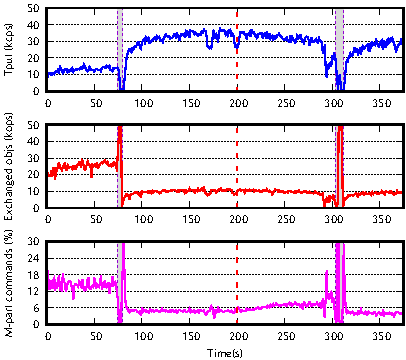
\includegraphics[width=\textwidth]{./figures/experiments/dynastar/chirper-celeb-dynastar-no-oracle.pdf}
    \caption{}
  \end{subfigure}
  \begin{subfigure}{.48\textwidth}
    \centering
    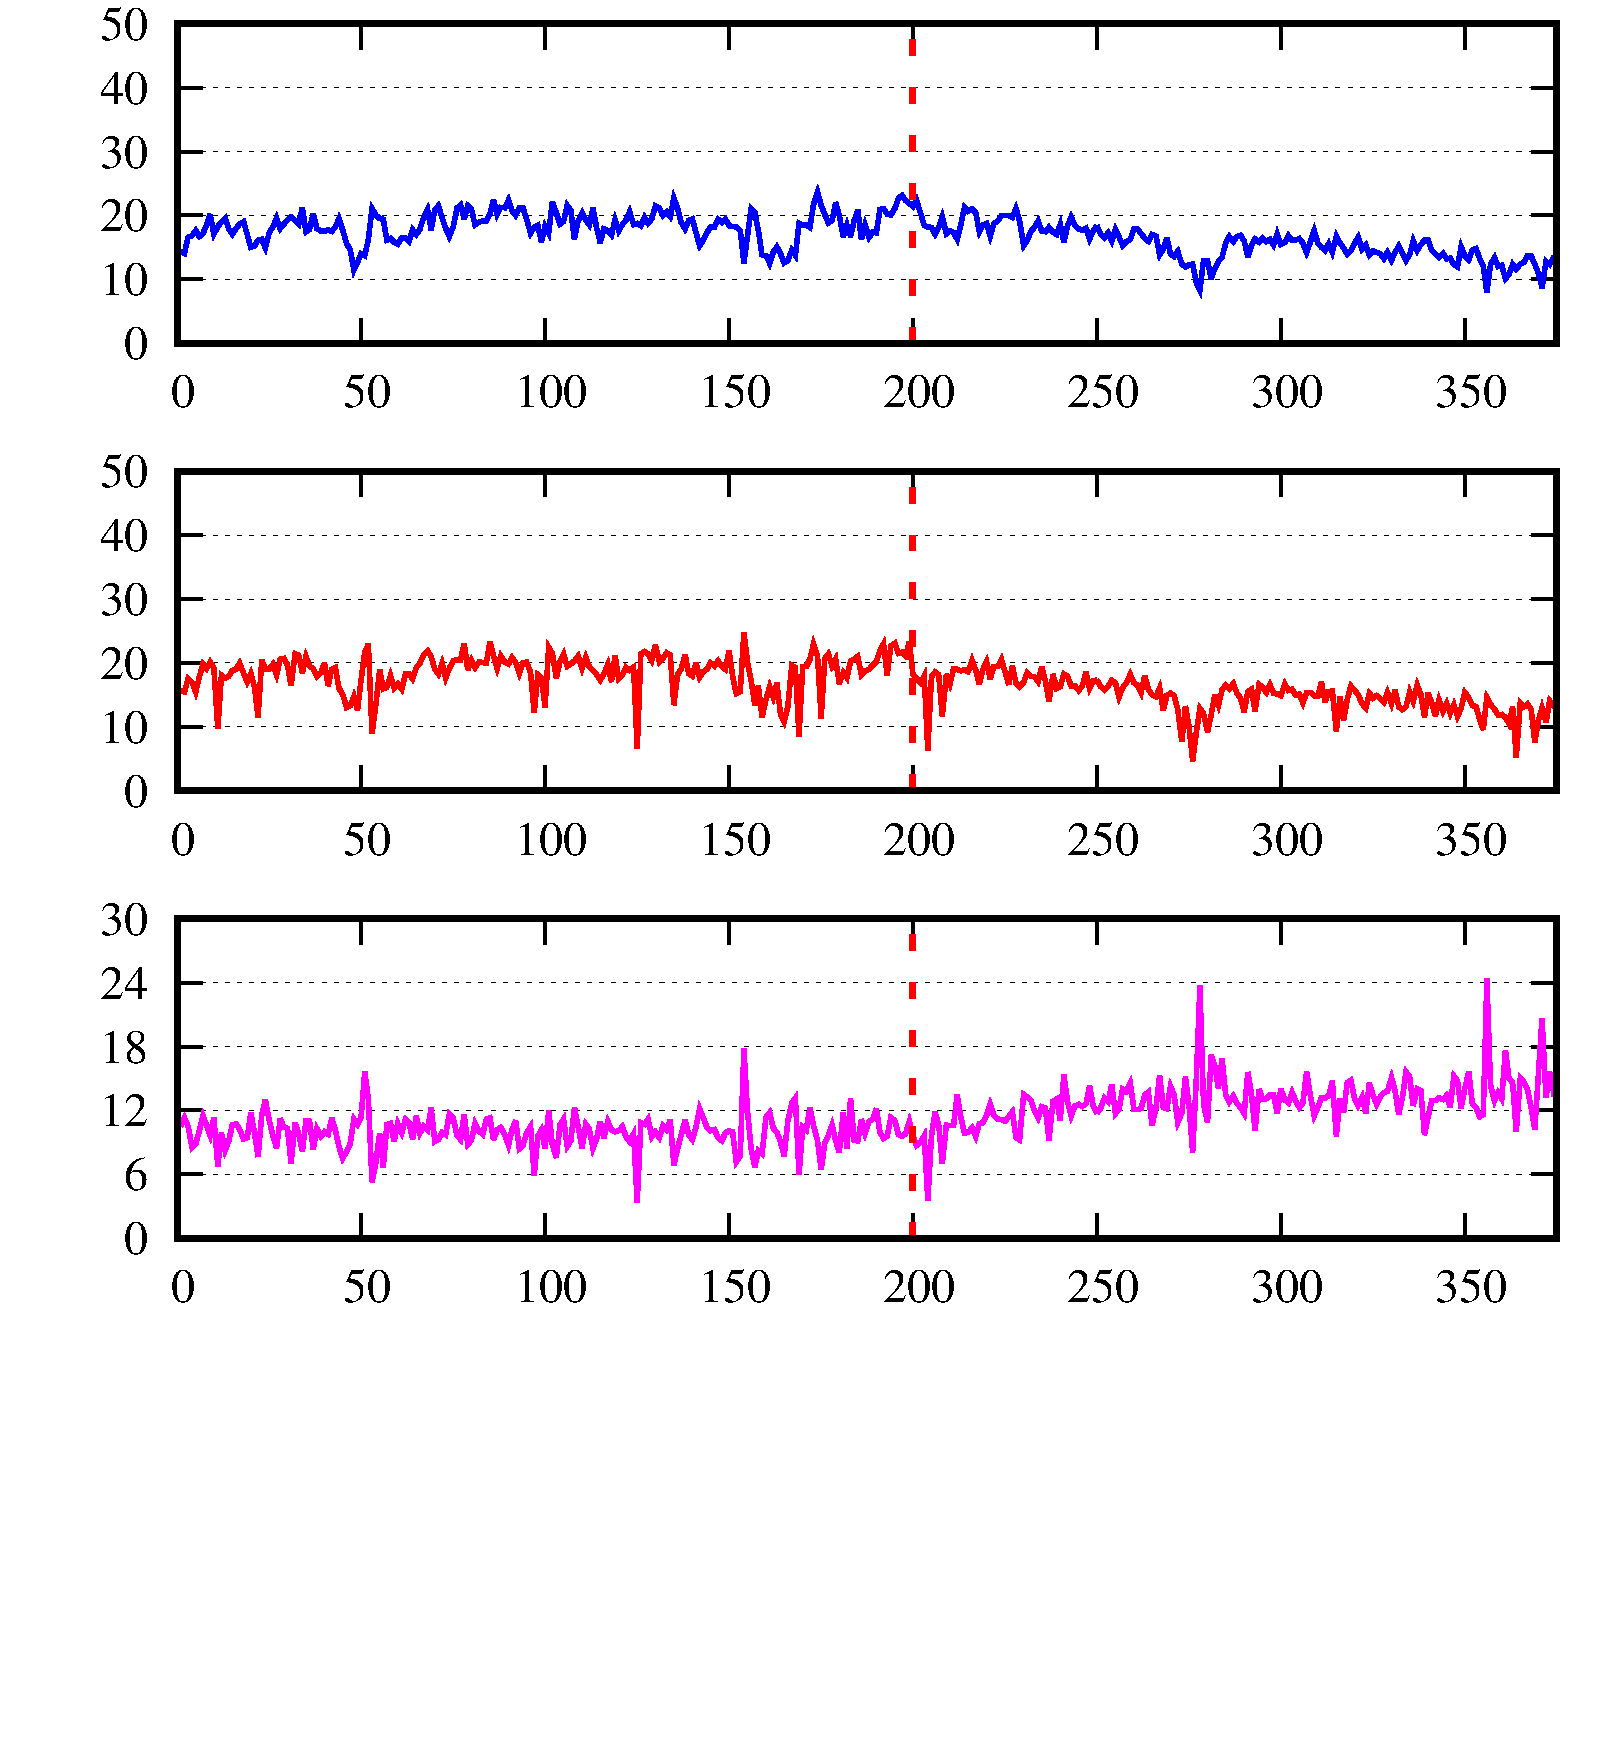
\includegraphics[width=\textwidth]{./figures/experiments/dynastar/chirper-celeb-ssmr.pdf}
    \caption{}
  \end{subfigure}
  \caption{Repartitioning a dynamic workload with \dynastar~(a) and S-SMR*
  without repartitioning (b).}%
  \label{fig:socialcelebrity}
\end{figure*}

At the beginning of the experiment, \dynastar performance was not as good as
S-SMR* (i.e., lower throughput, higher number of percentage of multi-partition
commands, and higher number of exchanged objects), because S-SMR* started with
an optimized partitioning, while \dynastar started with a random partitioning.
After 50 seconds, \dynastar triggered the repartitioning process, which led to
an optimized location of data. Repartitioning helped reduce the percentage of
multi-partition commands to 10\%, and thus increased the throughput. After the
repartitioning, \dynastar outperforms S-SMR* with the optimized partitioning.
After 200 seconds, the network started to change its structure, as many users
started to follow a celebrity, and created more edges between nodes in the
graph. Both \dynastar and S-SMR suffered from the change, as the rate of
multi-partition command increased, and the throughput decreased. However, when
the repartitioning takes place in \dynastar, around 300 seconds into the
execution, the previously user mapping got a better location from the oracle,
which adapted the changes. After the repartitioning, the objects are moved to a
better partition, with a resulting increase in throughput.

Figure~\ref{fig:dynastar-socialcdf} shows the cumulative distribution functions (CDFs) of
latency for the mix workload of \dynastar and S-SMR* on different
configurations. The results suggest that S-SMR* achieves lower latency than
\dynastar for 80\% of the load. This is expected, as for multi-partition
commands, partitions in \dynastar have to send additional data to return objects
to their original location after command execution .

\begin{figure*}[ht!]
  \centering
  \begin{subfigure}{0.48\columnwidth}
    \centering
    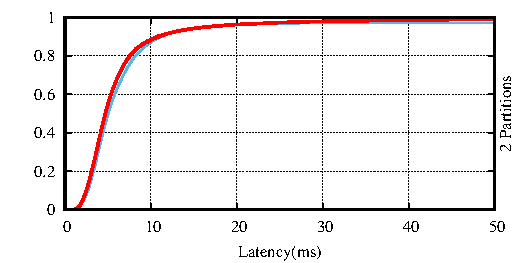
\includegraphics[width=\textwidth]{./figures/experiments/dynastar/chirper-latency-cdf-2p.pdf}
%    \caption{}
  \end{subfigure}
  \begin{subfigure}{0.48\columnwidth}
    \centering
    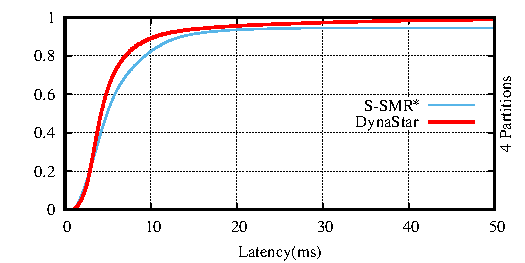
\includegraphics[width=\textwidth]{./figures/experiments/dynastar/chirper-latency-cdf-4p.pdf}
%    \caption{}
  \end{subfigure}
  \begin{subfigure}{0.48\columnwidth}
    \centering
    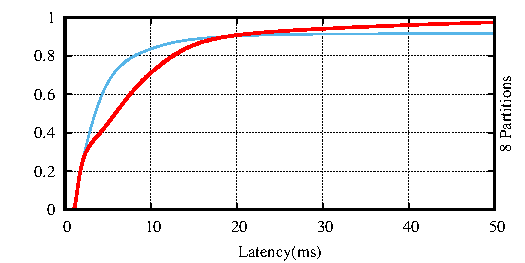
\includegraphics[width=\textwidth]{./figures/experiments/dynastar/chirper-latency-cdf-8p.pdf}
%    \caption{}
  \end{subfigure}
  \begin{subfigure}{0.48\columnwidth}
    \centering
    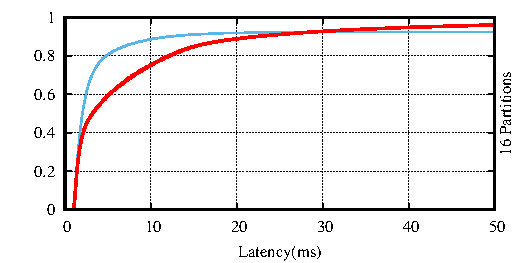
\includegraphics[width=\textwidth]{./figures/experiments/dynastar/chirper-latency-cdf-16p.pdf}
%    \caption{}
  \end{subfigure}
  \caption{Cumulative distribution function (CDF) of latency for mix workloads on different partitioning configurations.}
  \label{fig:dynastar-socialcdf}
\end{figure*}


Table ~\ref{table:dynastar-socialsnapshot} shows the throughput of each
partition when the system reached the maximum throughput at the time 180.
Although the objects were evenly distributed among partitions, there was still a
skew in the load of the system, e.g., partition 1 and 2 served more commands
than the other partitions. This happened because of the skew in the access
pattern: some users were more active and posted more than the others,
% thus the requests that sent to their servers are more than to other servers.
thus some servers receive more requests than the other servers.

\begin{table}[htp]
\caption{Average load at partitions at peak throughput.}
\label{table:dynastar-socialsnapshot}
\begin{adjustbox}{max width=\columnwidth}
\vspace{10mm}
\begin{tabular}{|c|c|c|c|}
\hline
Partition & Tput & M-part commands per sec & Exchanged objects per sec \\ \hline
1         & 12766      & 887                      & 3907              \\ \hline
2         & 11790      & 643                      & 3036              \\ \hline
3         & 6775       & 440                      & 1503              \\ \hline
4         & 6458       & 400                      & 1490              \\ \hline
\end{tabular}
\vspace{10mm}
\end{adjustbox}
\end{table}

\subsection{The performance of the oracle}

\dynastar  uses an oracle that maintains a global view of the workload graph.
The oracle allows \dynastar to make better choices about data movement,
resulting in overall better throughput and lower latency. However, introducing a
centralized component in a distributed system is always a cause for some
skepticism, in case the component becomes a bottleneck, or a single point of
failure. To cope with failures, the oracle is implemented as a replicated
partition.

The oracle keeps a mapping of objects to partitions and the relations between
objects. The size of the mapping depends on the complexity and the granularity
of the graph. In the social network dataset, where each user is modeled as an
object in the workload graph, the graph uses 1.5 GB of the oracle's memory. In
the TPC-C experiments, only district and warehouse objects are in the workload
graph; thus, the oracle only needs 1 MB of memory to store the graph for each
warehouse.

We conducted experiments to evaluate if the \dynastar oracle is a bottleneck
to system performance. The results show that the load on the oracle is low,
suggesting that \dynastar scales well. The first experiment assesses the
scalability of the METIS algorithm only. We measured the time to compute the
partitioning solution, and the memory usage of the algorithms for increasingly
large graphs. The results, depicted in Figure~\ref{fig:metis_size_time}, show
that METIS scales linearly in both memory and computation time on graphs of up
to 10 million vertices.

\begin{figure}[ht!]
  \centering
    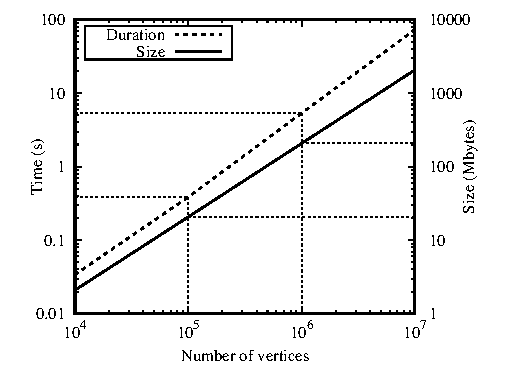
\includegraphics[width=0.7\columnwidth]{./figures/experiments/dynastar/metis_size_time}
	\caption{METIS processor and memory usage.}
	\label{fig:metis_size_time}
\end{figure}

\begin{figure}[ht!]
  \centering
    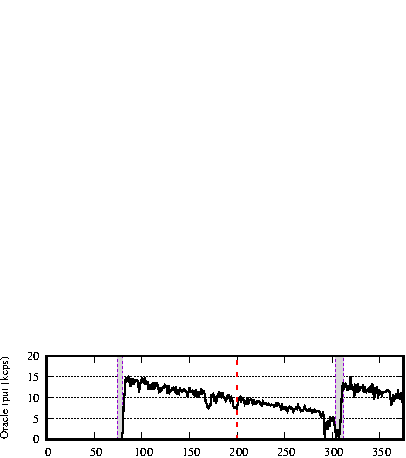
\includegraphics[width=0.8\columnwidth]{figures/experiments/dynastar/chirper-celeb-dynastar-oracle.pdf}
  \caption{Queries sent to oracle in the social network service}
  \label{fig:socialcelebrity-oracle}
\end{figure}


The second experiment evaluates the oracle in terms of the number of queries
sent to the oracle over time. The results shown in the bottom chart in the
Figure~\ref{fig:socialcelebrity-oracle} suggest that the oracle would not become a
bottleneck. The number of queries processed to the oracle is zero at the
beginning of the experiment, as the clients have cached the location of all
objects. After 80 seconds, the repartitioning was triggered, making all cached
data on clients invalid. Thus the throughput of queries at the oracle increases,
when clients started asking for new location of variables. However, the load
diminishes rapidly and gradually reduce. This is because access to the oracle is
necessary only when clients have an invalid cache or when a repartition happens


\section{Conclusion}
\label{sec:dynastar-conclusion}

In this chapter, we present \dynastar, a partitioning strategy for scalable state
machine replication. \dynastar is inspired by DS-SMR, a decentralized dynamic
scheme of \dssmr. Differently from DS-SMR, however, \dynastar performs well in
all workloads evaluated. When the state can be perfectly partitioned, \dynastar
converges more quickly than DS-SMR; when partitioning cannot avoid
cross-partition commands, it largely outperforms DS-SMR. The key insights of
\dynastar are to build a workload graph on-the-fly and use an optimized
partitioning of the workload graph, computed with an online graph partitioner,
to decide how to efficiently move state variables. The chapter describes how one
can turn this conceptually simple idea into a system that sports performance
close to an optimized (but impractical) scalable system.



%!TEX root =  main.tex
\chapter[Related works]{Related works}
\label{sec:rw}

In this chapter, we review related work on optimizing and scaling state machine
replication, partitioning application state, and optimize graph partitioning.

\paragraph{Consensus and state machine replication}
State machine replication (SMR) was first introduced by Leslie Lamport as an
example in ~\cite{Lam78}. Schneider \cite{Sch90} then gave a more systematic
approach to the design and implementation of SMR protocols. Util now SMR have
become a well-known approach to replication and has been extensively studied
~\cite{Kapritsos:2012um, Kotla:2004ep, santos2013htsmr}. SMR provides strong
consistency guarantees, which come from total order and deterministic execution
of commands. Deterministic execution is usually ensured by having every replica
execute commands sequentially. Traditional consensus based SMR repeatedly run
multiple instances of a consensus protocol to allow replicas to reach an agreed
order of commands. The best-known consensus algorithm is the Paxos protocol by
Lamport \cite{Lam98}. Raft \cite{184040}, a Paxos alternative also
implements consensus-based SMR, and it is suggested to be easier to understand
(than Paxos) from an engineering point of view.

\paragraph{Optimizing ordering protocol}

Even though increasing the performance of state machine replication is
non-trivial, different techniques have been proposed for achieving scalable
systems, such as optimizing the propagation and ordering of commands. This
allows the ordering layer (i.e., the underlying atomic broadcast algorithm) to
be itself also scalable. For instance, Kapritsos and
Junqueira~\cite{kapritsos2010scalable} propose to divide the ordering of
commands between different clusters: each cluster orders only some requests, and
then forwards the partial order to every server replica, which then merges the
partial orders deterministically into a single total order that is consistent
across the system. In S-Paxos~\cite{biely2012spaxos}, Paxos~\cite{Lam98} is used
to order commands, but it is implemented in a way such that the task of ordering
messages is evenly distributed among replicas, as opposed to having a leader
process that performs more work than the others and may eventually become a
bottleneck.

\paragraph{Parallelizing execution of commands}

Multi-threaded execution is a potential source of non-determinism, depending on
how threads are scheduled to be executed in the operating system. However, some
works have proposed multi-threaded implementations of state machine replication,
circumventing the non-determinism caused by concurrency in some way. In
\cite{santos2013htsmr}, for instance, the authors propose organizing each
replica in multiple modules that perform different tasks concurrently, such as
receiving messages, batching, and dispatching commands to be executed. The
execution of commands is still sequential, but the replica performs all other
tasks in parallel. In CBASE~\cite{Kotla:2004ep}, a parallelizer module uses
application semantics to determine which commands can be executed concurrently
without reducing determinism (e.g., read-only commands, which can be executed in
any order relative to one another). In Eve~\cite{Kapritsos:2012um}, commands are
tentatively executed in parallel. After the parallel execution, replicas verify
whether they reached a consistent state; if not, commands are rolled back and
re-executed sequentially.

\paragraph{Weakening consistency guarantees}

Many database replication schemes aim at achieving high throughput by relaxing
consistency, that is, they do not ensure linearizability. In deferred-update
replication \cite{chundi96dur, kobus2013hybrid, sciascia2012sdur, SousaOMP01},
replicas commit read-only transactions immediately, not always synchronizing
with each other. Although this indeed improves performance, it allows
non-linearizable executions. Database systems usually ensure serializability
\cite{BHG87} or snapshot isolation \cite{LinKJPA09}, which do not take into
account real-time precedence of different commands among different clients. For
some applications, these consistency levels may be enough, allowing the system
to scale better, but services that require linearizability cannot be implemented
with such techniques.

\paragraph{Partitioning application state}
Partitioning the state of a replicated service is conceptually similar to
partial replication of databases. Efforts to make linearizable systems scalable
have been made in the past~\cite{bezerra2014ssmr, corbett2013spanner,
Glendenning:2011kj, Marandi:2011dj}.  In Scatter~\cite{Glendenning:2011kj}, the
authors propose a scalable key-value store based on DHTs, ensuring
linearizability, but only for requests that access the same key. In the work of
Marandi et al~\cite{Marandi:2011dj}, variant of SMR is proposed in which data
items are partitioned but commands have to be totally ordered.
Spanner~\cite{corbett2013spanner} is a leader-leased, Paxos based system that
use TrueTime-accurate clock synchronization that require special hardwares to
improve geo-distributed read performance. Spanner uses a separate Paxos group
per partition and synchronized clocks to ensure strong consistency across
partitions. Although the authors say that Spanner works well with GPS and atomic
clocks, if clocks become out of synch beyond tolerated bounds, correctness is
not guaranteed. $M^2Paxos$~\cite{7579738} proposes a scheme where leases are
used instead of partitions owning objects, but assumes full state replication.
\ssmr{}~\cite{bezerra2014ssmr} ensures consistency across partitions without any
assumption about clock synchronization, but relies on a static partitioning of
the state. \dssmr{}~\cite{le2016dssmr} extends \ssmr\ by allowing state
variables to migrate across partitions in order to reduce multi-partition
commands. However, \dssmr{} implements repartitioning in a very simple way that
does not perform very well in scenarios where the state cannot be perfectly
partitioned. \dynastar\ improves on \dssmr\ by employing well-known graph
partitioning techniques to decide where each variable should be. Moreover,
\dynastar\ dilutes the cost of repartitioning by moving variables on-demand,
that is, only when they are accessed by some command.

\paragraph{Optimize graph partitioning}

Graph partitioning is an interesting problem with many proposed
solutions~\cite{Abou-Rjeili:2006,hendrickson2000graph,kernighan1970efficient,7004087}.
In this work, we do not introduce a new graph partitioning solution, but instead
we use a well-known one (METIS~\cite{Abou-Rjeili:2006}) to partition the state
of a service implemented with state machine replication. Similarly to
\dynastar{}, Schism~\cite{curino2010sch} and Clay~\cite{SerafiniTEPAS16} also
use graph-based partitioning to decide where to place data items in a
transactional database. In either case, not much detail is given about how to
handle repartitioning dynamically without violating consistency. Turcu et al.
~\cite{7004087} proposed a technique that reduces the amount of cross-partition
commands and implements an advanced transaction routing.
Sword~\cite{quamar2013sword} is another graph-based dynamic repartitioning
technique. It uses a hyper-graph partitioning algorithm to distribute rows of
tables in a relational database across database shards. Sword does not ensure
linearizability and it is not clear how it implements repartitioning without
violating consistency. E-Store~\cite{taft2014est} is yet another repartitioning
proposal for transactional databases. It repartitions data according to access
patterns from the workload. It strives to minimize the number of multi-partition
accesses and is able to redistribute data items among partitions during
execution. E-Store assumes that all non-replicated tables form a tree-schema
based on foreign key relationships. This has the drawback of ruling out
graph-structured schemas and \mbox{$m$-$n$} relationships. \dynastar\ is a more
general approach that works with any kind of relationship between data items,
while also ensuring linearizability.

Some replication schemes are ``dynamic'' in that they allow the membership to be
reconfigured during execution (e.g.,
\cite{birman2010dsr,dustdar2007soc,guessoum2003dar}). For instance, a multicast
layer based on Paxos can be reconfigured by adding or removing acceptors. These
systems are dynamic in a way that is orthogonal to what \dynastar\ proposes.

\dynastar\ consists of allowing the \emph{state partitioning}, that is, which
state variables belong to which partition, to change dynamically. The greatest
challenge that is addressed by \dynastar\ is how to provide such a solution,
with a dynamic partitioning oracle, while ensuring a very strong level of
consistency (linearizability), as variables are created, deleted, and moved
across partitions, based on the access patterns of the workload.



\chapter[Conclusion]{Conclusion}

In this thesis we have investigated the problem of scaling state machine
replication, focusing on understanding the performance characteristics and
proposing techniques to achieve a scalable performance.


We have proposed here \dynastar, a novel state machine replication approach that
allows state machine replication to scale by dynamically adapting to the
workload, while still ensuring strong consistency. This is a work in progress,
though, and thus needs to be further elaborated. For this purpose, a few points
need to be addressed:

\begin{itemize}

    \item[i)]\emph{Decentralized partitioning:}
    Even though defining optimized partitioning by using a centralized oracle
    shows its advantages over the decentralized approach, the oracle is still
    prone to becoming a bottleneck as the workload becomes bigger or less
    clustered, since it has to handle more queries from clients. A decentralized
    graph partitioning approach could help solve this problem.

    \item[ii)]\emph{Reconfiguring partitions:}
    In \dynastar, we considered a fixed number of partitions. Changing the
    number of partitions in a \dynastar\ deployment while the system is running,
    is not a trivial problem to solve efficiently. Ideally \dynastar\ could
    allow application's state to shrink or expand to fit into a partitioning
    configuration with more or less partitions, in order to add or remove a
    partition dynamically.

\end{itemize}

Furthermore, \dynastar currently requires clients to explicitly send specific
commands to create workload graph (e.g., creating vertices or edges between
vertices). We plan to create a development environment, in the form of a
programming library, that allows the application designer to focus on the
application logic, rather than on graph partitioning and remote execution
details. The creation of the graph, handling of state partitioning and
distributed execution of commands will be handled internally by the library.


\include{11-appendix}

\backmatter

\fxnote{removing DOI and URL for consistency}

\bibliographystyle{dcu}
\bibliography{references}
\cleardoublepage
% \theindex %optional, use only if you have an index, must use
	  %\makeindex in the preamble

\end{document}